%TODO REMARQUES GENERALES DE SEAN
% Ne dis pas ce que tu ne peux pas faire mais ce que tu peux (avec limitations expliquées)
% Mélanger les chapitres 3 et 4. Faire un chapitre 3 concentré sur le disque et un chapitre 4 concentré sur les mécanismes de formations
% Dans la section 4.2, faire plusieurs disques et montrer les différences

\section{Les résonances dans un disque protoplanétaire}
À cause de la migration, l'apparition de résonances de moyen mouvement est favorisée durant la formation planétaire. C'est un phénomène qui tient un rôle majeur durant la formation. Après une brève description des résonances dans le cas général, nous étudierons les résonances dans le cas particulier (dissipatif) des disques de gaz. 

\subsection{Définition}\index{résonance!de Moyen Mouvement}\index{Mean Motion Resonance|see{résonance}}
Les \gras[resonance@résonance]{résonances de moyen mouvement} sont des configurations orbitales particulières de deux planètes
dans lesquelles il existe un lien entre les périodes orbitales des planètes. Exemple, si deux planètes sont en résonance
\MMR{3}{2}, ça signifie que la planète interne effectuera 3 orbites pendant que la planète externe en effectuera 2.

Ces configurations particulières confèrent une stabilité accrue aux planètes. Plus la résonance est forte et plus il sera
difficile pour les planètes d'en sortir.

\bigskip

On met généralement une résonance sous la forme \MMR{(p+q)}{p} où $p$ et $q$ sont des entiers. Cette forme permet de mettre en
évidence un des paramètres qui permet de rendre compte de la force de la résonance. En effet, plus $q$ est petit et plus la
résonance est forte. Ainsi, les résonances d'ordre 1 ($q=1$) sont les plus fortes. On dit que $q$ est l'ordre de la résonance
(plus l'ordre est petit et plus la résonance est forte). De même, $p$ est le degré de la résonance.

\begin{attention}
Mais ce n'est pas le seul paramètre à prendre en compte pour évaluer la force d'une résonance et je suis bien incapable de tous
les décrire.
\end{attention}

Pour une résonance \MMR{(p+q)}{p} on définit un certain nombre d'angles $\theta_i$ dits \gras[angle de résonance]{angles de
résonance} de la forme :
\begin{align}
\theta_{i+1} &=(p+q)\lambda_2 -p\lambda_1 - \left[i\varpi_{1} + (q-i)\varpi_2\right]
\end{align}
avec $i$ allant de $0$ à $q$ ; où $\lambda$ sont les longitudes moyennes, $\varpi$ les longitudes du péricentre et les indices
$1$ et $2$ se réfèrent respectivement à la planète interne et externe. Pour une résonance \MMR{(p+q)}{p} on a donc $q+1$ angles
de résonance.

Les angles de résonances mesurent l'angle entre les deux planètes au point de conjonction. Si un seul de ces angles est en
libration (oscillation autour d'une valeur moyenne) au lieu de circuler librement de $0$ à $2\pi$ alors on dit que les planètes
sont en résonances. Le nombre d'angles en libration permettra aussi d'avoir une idée de la force de la résonance.

\begin{exemple}
Soit une résonance \MMR{7}{2}, les angles de résonances sont :
\begin{align*}
\theta_1 &= 7 \lambda_2 -2\lambda_1 - 5 \varpi_1\\
\theta_2 &= 7 \lambda_2 -2\lambda_1 - \left( 4 \varpi_1 + 1\varpi_2 \right)\\
\theta_3 &= 7 \lambda_2 -2\lambda_1 - \left( 3 \varpi_1 + 2\varpi_2 \right)\\
\theta_4 &= 7 \lambda_2 -2\lambda_1 - \left( 2 \varpi_1 + 3\varpi_2 \right)\\
\theta_5 &= 7 \lambda_2 -2\lambda_1 - \left( 1 \varpi_1 + 4\varpi_2 \right)\\
\theta_6 &= 7 \lambda_2 -2\lambda_1 - 5 \varpi_2
\end{align*}
\end{exemple}

\begin{remarque}
Les \gras[kirkwood@Kirkwood!lacunes de]{lacunes de Kirkwood} font elles aussi intervenir des résonances mais contrairement à ce
qu'on pourrait penser, ces résonances avec Jupiter sont des zones déplétées en astéroïdes. 

La résonance imposte une valeur de $a$, mais des échanges sont possibles entre les deux corps en résonance et il est possible
que par ce biais l'excentricité puisse augmenter, et ainsi dépléter la lacune de kirkwood en favorisant les collisions entre les
objets en résonance et les autres qui sont dans la ceinture.
\end{remarque}


%TODO MMR : lire a thorough analysis of the dunamics involved the reader should consult (Murray & Dermott, 1999)
%TODO cité depuis chapitre 8 resonant perturbations : 
% useful reviews of the subject, particularly in the context of orbital evolution through resonance, have been given by
%Greenberg (1977), Peale (1986) and Malhotra (1988).
%TODO 
\subsection{Résonances et excentricité}
Cela dépend de l'ordre et du degré de la résonance, mais les perturbations gravitationnelles mutuelles de deux corps en
résonance de moyen mouvement engendrent des modifications des éléments orbitaux de ces derniers. 

En particulier, l'excentricité de deux corps en résonance a tendance à varier augmenter au cours du temps \citep[eq.
(8.29)]{murray2000solar}. 

Nous n'allons pas détailler ici le fonctionnement précis des résonances. Plusieurs auteurs traitent de ce sujet
\citep{greenberg1977orbit, peale1986orbital, malhotra1988phd}. C'est un sujet extrêmement complexe, que je ne maitrise
absolument pas dans les détails. De plus, dans le cadre de notre étude de la formation des planètes, nous sommes dans un cas un
peu différent. Les résonances entre planète ont lieu dans un système dissipatif, le disque protoplanétaire, qui agit sur les
éléments orbitaux, par exemple en amortissant l'excentricité et l'inclinaison des planètes.

Il est difficile de prendre pour exemple les cas N-corps classiques et essayer de les appliquer dans le disque de gaz. Dans
notre cas, l'amortissement de $e$ et $I$ par le disque stabilise les résonances, empêchant les résonances normalement instables
de se briser. Bien entendu, les résonances se brisent dans nos systèmes en formation, mais dans des cas beaucoup plus extrêmes,
notamment quand on a une chaîne de résonance contenant plusieurs corps, tous en résonance. 

\subsection{Stabilité et ordre des résonances}
\reffig{fig:MMR_statistique} montre l'influence du degré de la résonance sur l'excentricité des deux planètes mises en jeu. On
constate tout d'abord que sur 250 simulations effectuées, aucune ne présente des résonances d'ordre $q\neq 1$. Dans le cas de la
migration, où les planètes veulent sortir de la résonance au travers de leur migration différentielle, seules les migration
d'ordre 1 sont assez fortes pour survivre. 


\begin{figure}[htbp]
\centering
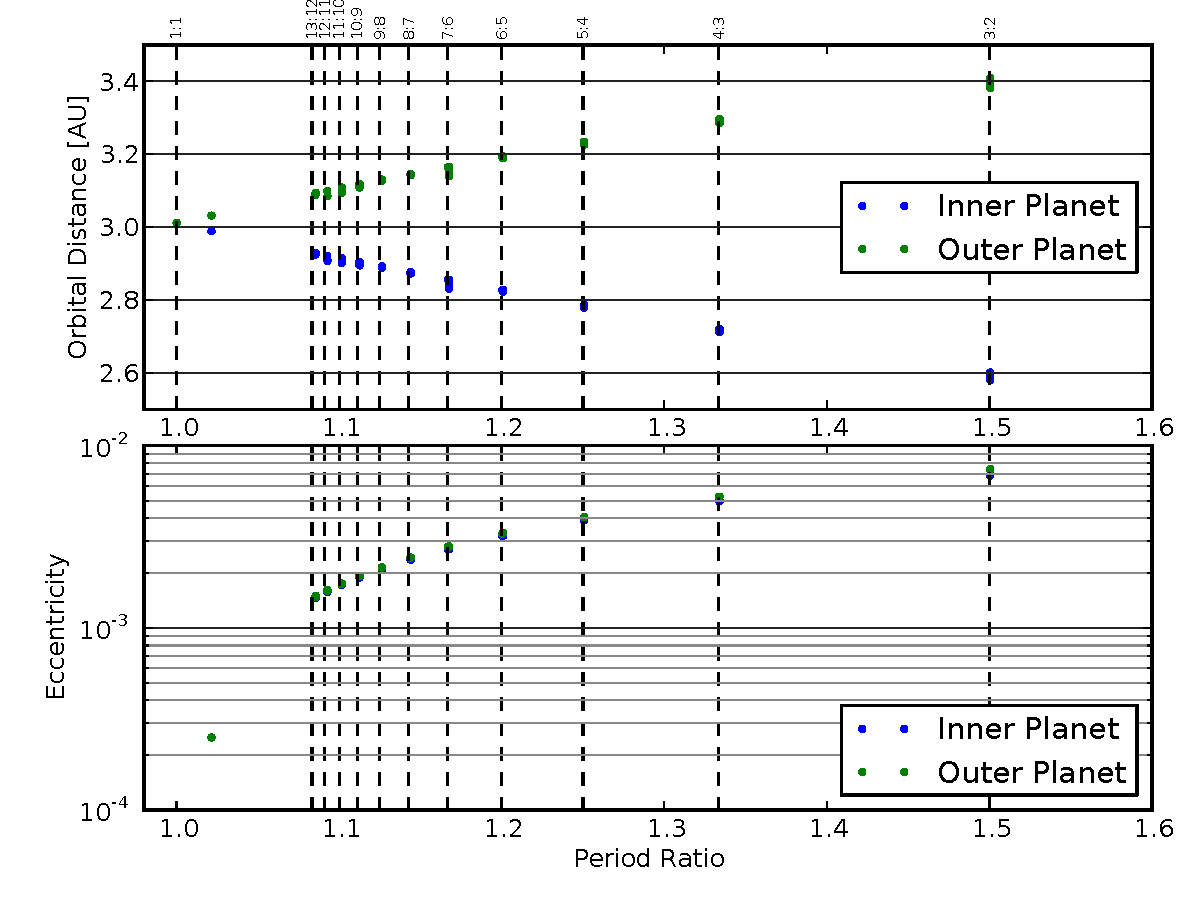
\includegraphics[width=0.75\linewidth]{figure/MMR_statistique.pdf}
\caption{Illustration des différentes résonances possibles et de l'augmentation de l'excentricité qu'elles entrainent. Chaque
simulation contenait deux planètes de $1\mearth$ aléatoirement réparties entre $1$ et $10\unit{AU}$. Chaque point correspond à
une planète. En haut, en fonction du rapport de période, la position finale des planètes est
représentée. En bas, l'excentricité des planètes en fonction du rapport de période avec l'autre planète du système. Une zone de
convergence artificielle à $3\unit{UA}$ a été appliquée. Elle n'a pas d'importance particulier sinon de permettre la formation
de résonances, centrées autour de la même zone du disque, facilitant les études comparatives.}\label{fig:MMR_statistique}
\end{figure}

En fonction du degré de la résonance, l'excentricité des deux corps en résonance diffère. Contrairement à ce qu'on pourrait
penser, ce ne sont pas les résonances de degré élevés qui engendrent les excentricités les plus grandes, même si la distance
entre les deux corps diminue drastiquement. Ainsi, l'excentricité de deux corps sera plus grande s'ils sont en résonance
\MMR{3}{2} par rapport à une \MMR{9}{8}. Ceci vient du fait que même si les planètes sont plus éloignées, dans le cas d'une
résonance \MMR{3}{2}, les conjonctions à l'origine des perturbations gravitationnelles résonances sont beaucoup plus
fréquentes. L'augmentation de l'excentricité est donc beaucoup plus importante \citep{murray2000solar}. 

\subsection{Effet du rapport de masse}
%phd/MMR_mass_ratio
\begin{figure}[htbp]
\centering
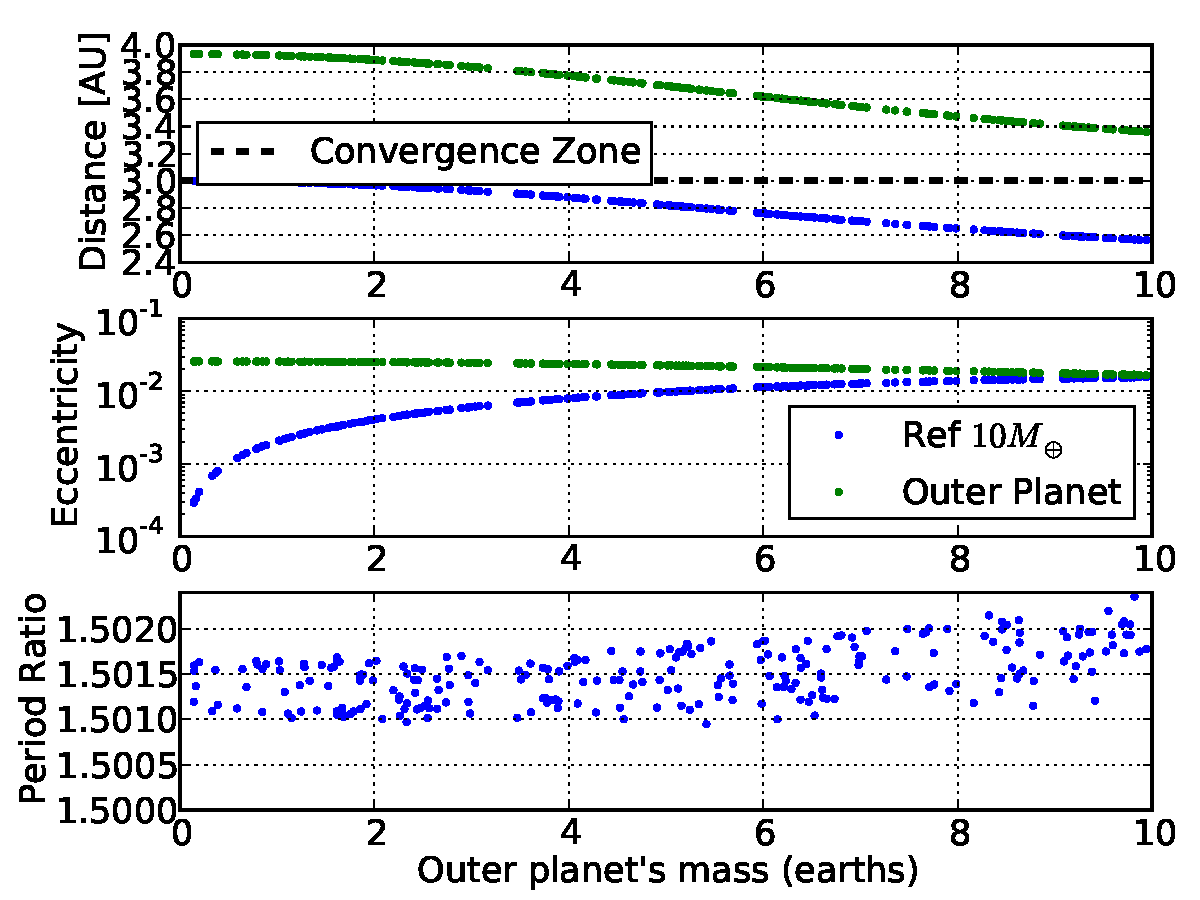
\includegraphics[width=0.75\linewidth]{figure/MMR_mass_ratio.pdf}
\caption{Résultat de 250 simulations où la première planète, de $10\mearth$ est à $3\unit{UA}$, sur
la zone de convergence artificielle. Une planète externe, placée à $4\unit{UA}$ a une masse
déterminée aléatoirement entre $0.1$ et $10\mearth$. Dans la totalité des simulations, les planètes
se placent en résonance \MMR{3}{2}.}\label{fig:MMR_mass_ratio}
\end{figure}

\reffig{fig:MMR_mass_ratio} se lit de gauche à droite, afin de voir l'effet de l'augmentation de la masse de la planète externe
sur la distance orbitale, l'excentricité et le rapport de périodes orbitales. 

Pour une seconde planète de $0.1\mearth$, on constate que la planète la plus massive se trouve à la position exacte de la
résonance, tandis que la planète externe reste bloquée à $4\unit{UA}$ environ. Les deux planètes ressentent un couple de
migration vers la zone de convergence à $3\unit{UA}$ mais l'inertie de la planète massive est beaucoup plus grande, raison pour
laquelle la planète de $10\mearth$ est à la zone de convergence, la planète de faible masse étant simplement bloquée dans la
résonance. 

On constate de plus qu'en raison de la très grande différence de masse, pour une même résonance l'excentricité des deux
planètes est très différente. La planète la plus massive a une excentricité extrêmement basse, cette dernière étant très peu
sensible aux perturbations de la planète de faible masse. À l'inverse, la planète peu massive est très sensible aux
perturbations de la plus grosse, et son excentricité est bien plus importante, plus de deux ordres de grandeur supérieure.

Pour cette planète externe de $0.1\mearth$ on remarque une dernière chose. Bien qu'en résonance \MMR32, le rapport de période
ne vaut pas exactement $1.5$ comme attendu, mais $1.503$. On retrouve là la divergence du rapport de période pour des
résonances dans un système dissipatifs \citep{batygin2013dissipative}. 

\bigskip

À mesure que l'on augmente la masse de la planète externe, cette dernière pousse petit à petit la planète interne, le rapport
de masse se rapprochant de $1$, elle a peu à peu suffisamment de force pour que l'équilibre des couples de migration se
traduise par une répartition des planètes autour de la zone de convergence. 

Dans le même temps, l'excentricité de la planète interne croit. À mesure que la masse de la planète externe augmente, les
perturbations qu'elle engendre sur l'autre planète augmentent également. Sa masse augmentant, elle devient légèrement moins
sensible aux perturbations de la planète interne et on constate une baisse ténue de l'excentricité de la planète externe. 

Enfin, on remarque que l'écart du rapport de période par rapport à la valeur attendue de $1.5$ pour une résonance \MMR32
augmente avec la masse du deuxième corps. En effet, à mesure que la masse de la planète externe augmente, l'amortissement de
l'excentricité induit par le disque devient plus efficace \citep[eq. (9)]{cresswell2008three}. 

\bigskip

Une fois que le rapport de masse est égal à 1, alors les planètes se placent de part et d'autre de la zone de couple nul, et
les excentricités induites par la résonances deviennent sensiblement égales.

\section{Zones de convergence et Résonances}
%TODO talk about the difference between mass dep and mass indep accretion, in particular the fact that planet of different
%masses migrate to different position has an influence on the convergent migration. 
% In particular, mass indep with linear migration can be equivalent to mass-indep with steep transition.
%TODO

Nous cherchons à comprendre comment l'accrétion est influencée par une zone de convergence. Cette convergence des embryons
planétaire vers une zone préférentielle ne résulte pas en la formation d'une super planète, résultat de la collision de tous les
embryons de la zone de convergence \citep{morbidelli2008building, sandor2011formation}. Au lieu de cela, les planètes
interagissent entre elles et sont piégées dans des résonances de moyen mouvement \reffig{fig:MMR_number}. 

\begin{figure}[htbp]
\centering
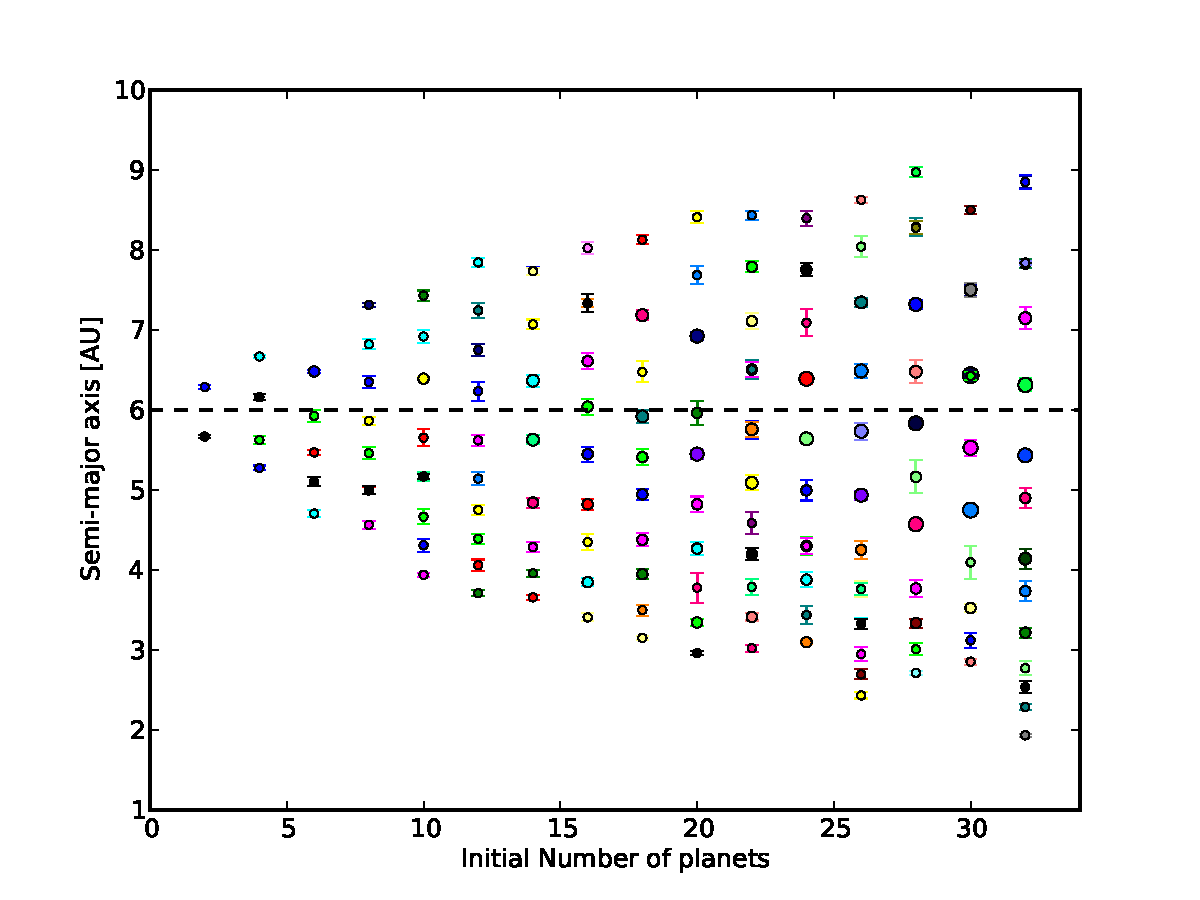
\includegraphics[width=0.75\linewidth]{figure/MMR_number.pdf}
\caption{Stabilisation d'un système planétaire autour d'une zone de convergence artificielle à $6\unit{UA}$ en fonction du
nombre de planètes qui le composent initialement. Les excentricités sont représentées par les barres d'erreurs. Le diamètre des cercles représentant les planètes est proportionnel à leur rayon (en considérant qu'elles ont toutes la même
densité).}\label{fig:MMR_number}
\end{figure}

De plus, les résonances de degré élevé sont favorisées. En effet, les perturbations sont fréquentes dans la chaîne de résonance dû au grand nombre de corps. Quand une résonance est brisée, les planètes ont tendance à se rapprocher à cause de la migration convergente, il est donc peu probable qu'elles atteignent de nouveau les rapports de périodes orbitales relativement élevés pour se placer en résonance \MMR21 ou \MMR32. 

\begin{figure}[htbp]
\centering
\subfloat[$N\simeq 15$]{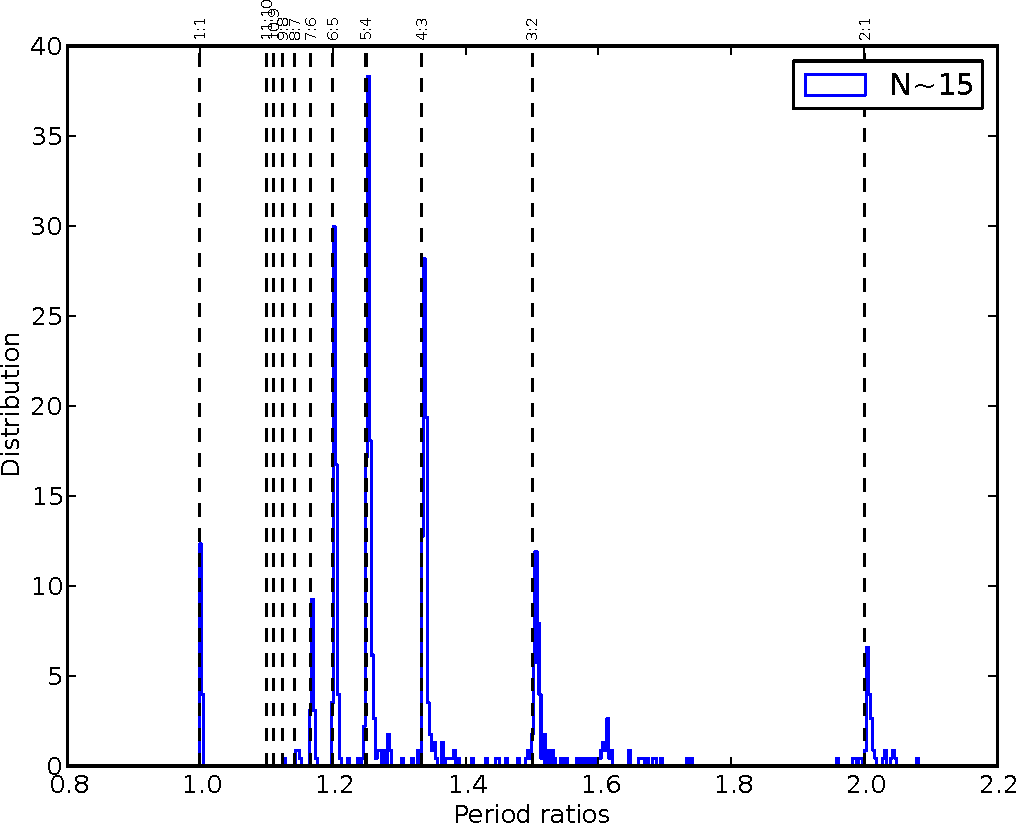
\includegraphics[width=0.49\textwidth]{%
figure/number_effect/N_15.pdf}}\hfill
\subfloat[$N\simeq 30$]{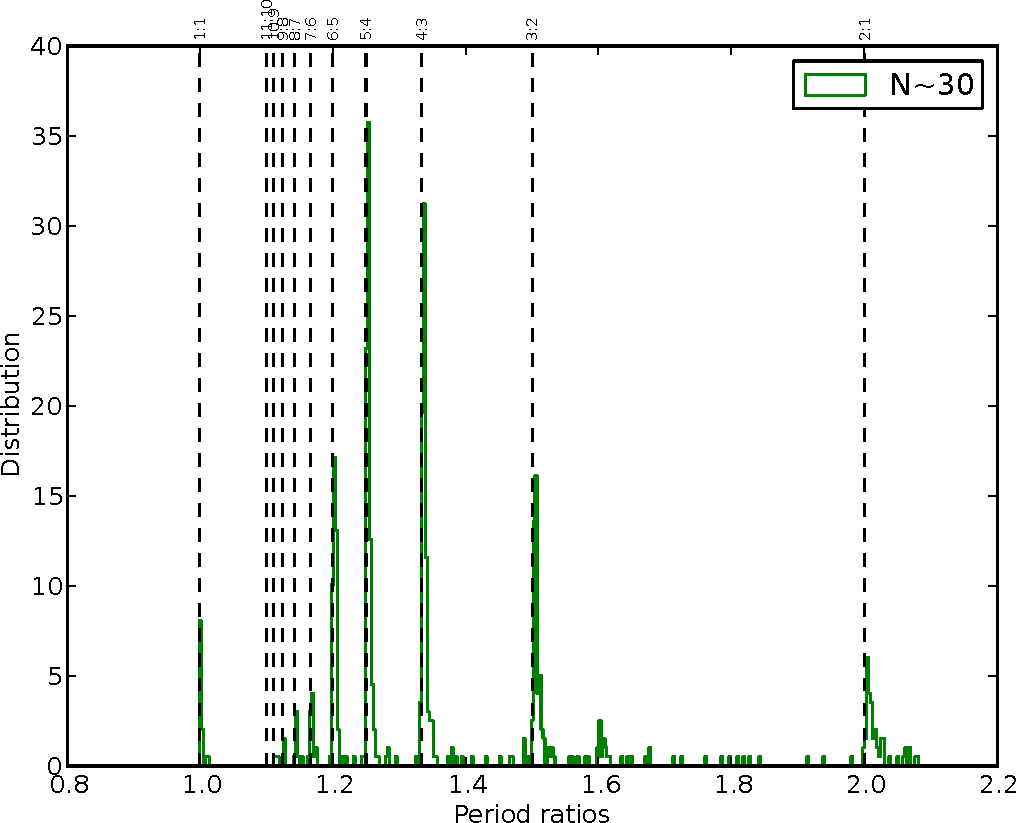
\includegraphics[width=0.49\textwidth]{figure/number_effect/N_30.pdf}}

\subfloat[$N\simeq 60$]{\label{fig:mass_effect}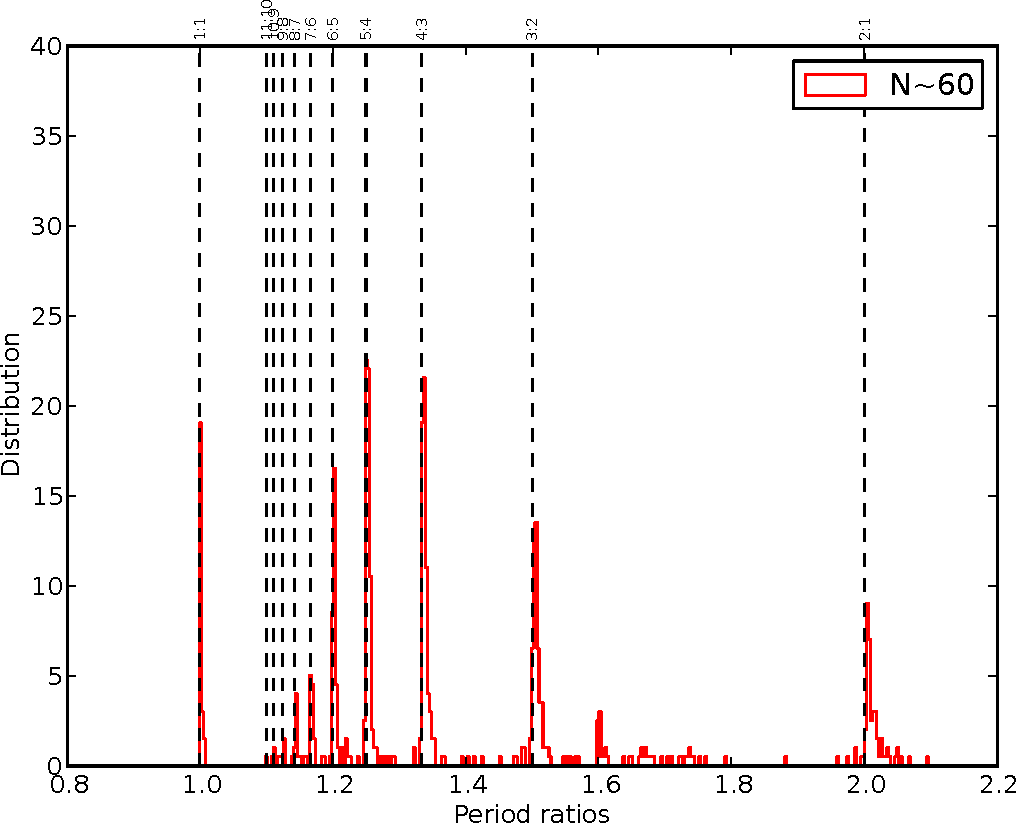
\includegraphics[width=0.49\textwidth]{%
figure/number_effect/N_60.pdf}}\hfill
\subfloat[Histogramme des masses]{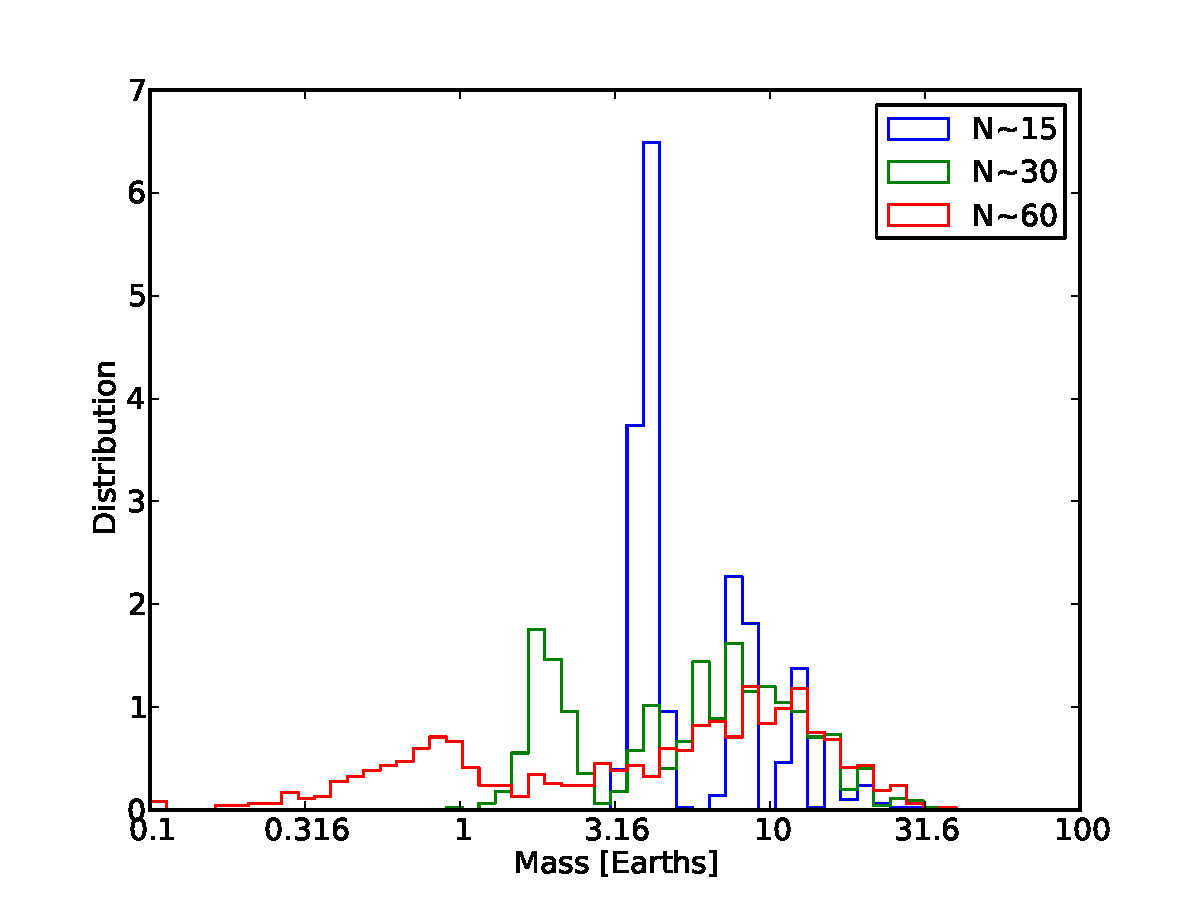
\includegraphics[width=0.49\textwidth]{figure/number_effect/number_effect_on_max_mass.pdf}}

\caption{Évolution des rapports de période orbitale et masses dans 100 systèmes planétaires où la masse totale est de $60\mearth$ mais où le nombre total d'embryons varie autour de valeurs moyennes différentes (15, 30 ou 60). }\label{fig:number_effect}
\end{figure}

Nous avons fixé la masse totale contenue dans les embryons planétaires initialement à $M_\text{tot}=60\mearth$. Les positions des planètes sont aléatoires et réparties uniformément entre $1$ et $10\unit{UA}$. Les orbites sont initialement quasi-circulaires et avec une inclinaison inférieure à $1^\circ$. Nous faisons évoluer ces systèmes pendant 10 millions d'années dans un disque où une zone de convergence artificielle est placée à $5\unit{UA}$. Nous souhaitons voir les interactions entre zone de convergence et résonances. 

De ces systèmes, nous créons trois sous-cas :
\begin{itemize}
\item Les planètes ont des masses aléatoires gaussiennes dont la moyenne vaut $\mu_m=1\mearth$ et l'écart-type vaut $\sigma_m=0.3\mearth$. Le nombre initial moyen de planètes par simulation est d'environ $N\sim 60$.
\item Les planètes ont des masses aléatoires gaussiennes dont la moyenne vaut $\mu_m=2\mearth$ et l'écart-type vaut $\sigma_m=0.3\mearth$. Le nombre initial moyen de planètes par simulation est d'environ $N\sim 30$.
\item Les planètes ont des masses aléatoires gaussiennes dont la moyenne vaut $\mu_m=4\mearth$ et l'écart-type vaut $\sigma_m=0.3\mearth$. Le nombre initial moyen de planètes par simulation est d'environ $N\sim 15$.
\end{itemize}

Pour chacun de ces trois cas, nous avons lancé 100 simulations. 

Les statistiques que nous obtenons sont compilées \reffig{fig:number_effect}. À mesure que le nombre de corps dans le système augmente, la compression de la chaîne de résonance augmente. Peu à peu, les résonances de degré élevé commencent à se peupler. Les résonances \MMR87 et \MMR98 très peu peuplées dans le cas $N\sim 15$ deviennent de plus en plus peuplées à mesure qu'on augmente le nombre de corps. Les résonances \MMR{10}{9} et \MMR{11}{10} qui n'étaient pas peuplées dans le cas $N\sim 15$ le sont propressivement quand on aumente $N$. Des planètes en résonances \MMR{10}{9} apparaissent dans le cas $N\sim 30$ et la résonance \MMR{11}{10} apparait dans le cas $N\sim 60$.

Enfin, il est à noter que les résonances de degré les plus bas se trouve généralement à l'extérieur de la chaîne de résonance. À l'inverse, les coorbites se trouvent préférentiellement au cœur de la chaîne de résonance, au plus proche de la zone de convergence où la compression est la plus grande. 

Quand on augmente le nombre d'embryons initiaux, vu que l'on travaille à masse totale constante, la masse de chaque embryon est statistiquement plus petite. Pour 15, 30 ou 60 embryons, les masses moyennes initiales sont respectivement $4$, $2$ et $1\mearth$. Sur \reffig{fig:mass_effect} nous voyons la répartition de la masse des planètes en fin de simulation en fonction du cas considéré ($N\sim 15$, 30 ou 60). Le premier pic de chaque cas représente les planètes qui n'ont pas eu de collisions tout au long de la simulation. Nous voyons donc bien que plus le nombre d'embryons augmente, plus la masse minimale d'une planète est petite (toute simulation confondues, parmis les 100 échantillons de systèmes planétaires). 

Quand le nombre d'embryons est très réduit ($N\sim 15$), l'histogramme des masses se réduit à une succession de pics car quelle que soit la masse moyenne de la gaussienne initiale l'écart-type était toujours de $\sigma_m = 0.3\mearth$. 

À l'inverse, quand le nombre d'embryons initiaux est grand ($N\sim 60$), la masse maximale tous systèmes planétaires confondus tend à être plus grande. Augmenter le nombre d'embryons, à masse totale constante, augmente le nombre de planètes en résonance ce qui augmente les perturbations gravitationnelles au sein de la chaîne de résonance. La probabilité de collisions et de coorbitaux augmente alors aussi, chaque sortie de résonance engendrant un épisode instable et chaotique pouvant déboucher soit vers une nouvelle capture en résonance, soit vers une collision, soit vers des coorbitaux. 

\section{Décalage de la Zone de Convergence}\label{sec:shifted_CZ}
Cette partie a fait l'objet d'un article, publié dans le journal Astronomy \& Astrophysics : \cite{cossou2013convergence}.

Une zone de convergence est une zone du disque agissant comme un piège à planète, la migration emmenant les planètes dans cette zone du disque où elles se stabilisent. Ici nous cherchons à montrer que dans le cas multi planétaire, les choses sont un peu différentes. Des planètes en résonance ne se comportent plus de la même manière, mais plutôt comme un système dans sa globalité, migrant dans une zone différente du disque.

\subsection{Introduction}
Des planètes de faible masse ($1-60\mearth$) interagissent avec le disque de gaz dans lequel elles se forment et génèrent des ondes de densité dans le disque \citep{goldreich1979excitation}. La planète elle même est influencée par cette onde de densité et migre par migration de Type I \citep{ward1997protoplanet}.

Dans les disques isothermes, la migration de Type I est gouvernée par le couple différentiel dû aux ondes de Lindblad et le couple de corotation. Pour les planètes, la migration qui en résulte est rapide et dirigée vers l'étoile centrale \citep{tanaka2002three}. Dans les disques radiatifs, un couple lié au gradient d'entropie apparait dans la zone en fer-à-cheval de la planète. Ce dernier peut contrebalancer le couple différentiel de Lindblad au point de transformer la migration vers l'intérieur précédemment présentée en migration vers l'extérieur. Ainsi, dans de tels disques, la migration peut être dirigée soit vers l'intérieur soit vers l'extérieur \citep{paardekooper2006halting, kley2008migration}. Ceci rend possible l'existence de zones dans les disques où la migration s'arrête. Ces dernières sont appelées zone de convergence \citep[CZs;][]{lyra2010orbital, mordasini2011application, paardekooper2011torque}.

\bigskip

À la zone de convergence, le couple de corotation (positif) compense exactement le couple différentiel de Lindblad (négatif). Ainsi, à la zone de convergence, une planète ne migre pas. Les zones de convergences pourraient ainsi concentrer les embryons planétaires et être le lieu de formation de planètes (ou cœurs) massives \citep{lyra2010orbital, horn2012orbital}. 

Cependant, durant leur migration vers la zone de convergence les planètes vont interagir entre elles et se placer en résonance de moyen mouvement (Mean Motion Resonance : MMR), s'opposant ainsi à l'accrétion illimitée de matière à la zone de convergence \citep{morbidelli2008building, sandor2011formation}. Malgré cela, des collisions ont bien lieu à la zone de convergence. Quand les embryons sont emprisonnés dans une chaine de résonance avec suffisamment de corps pour engendrer des perturbations, les résonances peuvent se briser et des collisions se produire entre les corps du système. De plus, la turbulence pourrait casser les résonances et augmenter le taux d'accrétion.

\bigskip

\cite{bitsch2010orbital} ont montré que le couple de corotation était atténué quand une planète avait une excentricité telle que son orbite oscille sur une distance de l'ordre de la demi-largeur de la zone fer-à-cheval $x_s$. 

Quand deux planètes sont en résonance à cause de la migration convergente, leurs excentricités sont excitées de manière continues malgré la présence du disque qui a tendance à amortir les excentricités et circulariser les orbites. \citep[par exemple ][]{cresswell2008three}. Ce phénomène devrait à son tour modifier le couple de corotation et ainsi modifier l'équilibre entre couple différentiel de Lindblad et couple de corotation. En conséquence, la migration de la planète elle-même devrait être modifiée.

\bigskip

Nous présentons des simulations de migration convergentes de planètes de faible masse ($M=1-10\unit{M_\oplus}$) dans un disque de gaz idéalisé (voir \refsec{sec:tanh_indep}). On utilise un modèle simplifié de rétroaction de l'excentricité sur le couple de corotation. Nous montrons que les planètes qui prises de manière isolé migrent à la zone de convergence, ne migrent plus au même endroit quand il y a plusieurs planètes. Au lieu de ça, elles migrent à une position d'équilibre décalée vers l'intérieur du disque qui correspond à une somme nulle des couples exercées sur le système. 

La position de cette zone d'équilibre dépend de l'excentricité maintenue par perturbation mutuelle de chaque planète constituante du système.

\subsection{Méthode}
On modélise une Zone de Convergence (CZ : Convergence Zone) artificielle, qui imite une zone de convergence indépendante de la masse, c'est à dire que la position de la zone de convergence est la même pour toutes les planètes quelle que soit leur masse \refsec{sec:CZ-types}. En particulier, on s'intéresse à la zone de convergence que l'on peut trouver à une transition d'opacité telle que celle représentée sur \reffig{fig:shifted_CZ_torque_prof}, où l'on peut voir un renversement brutal du couple, qui passe de positif à négatif \citep[voir par exemple ][]{masset2011type}.

\begin{figure}[htbp]
\centering
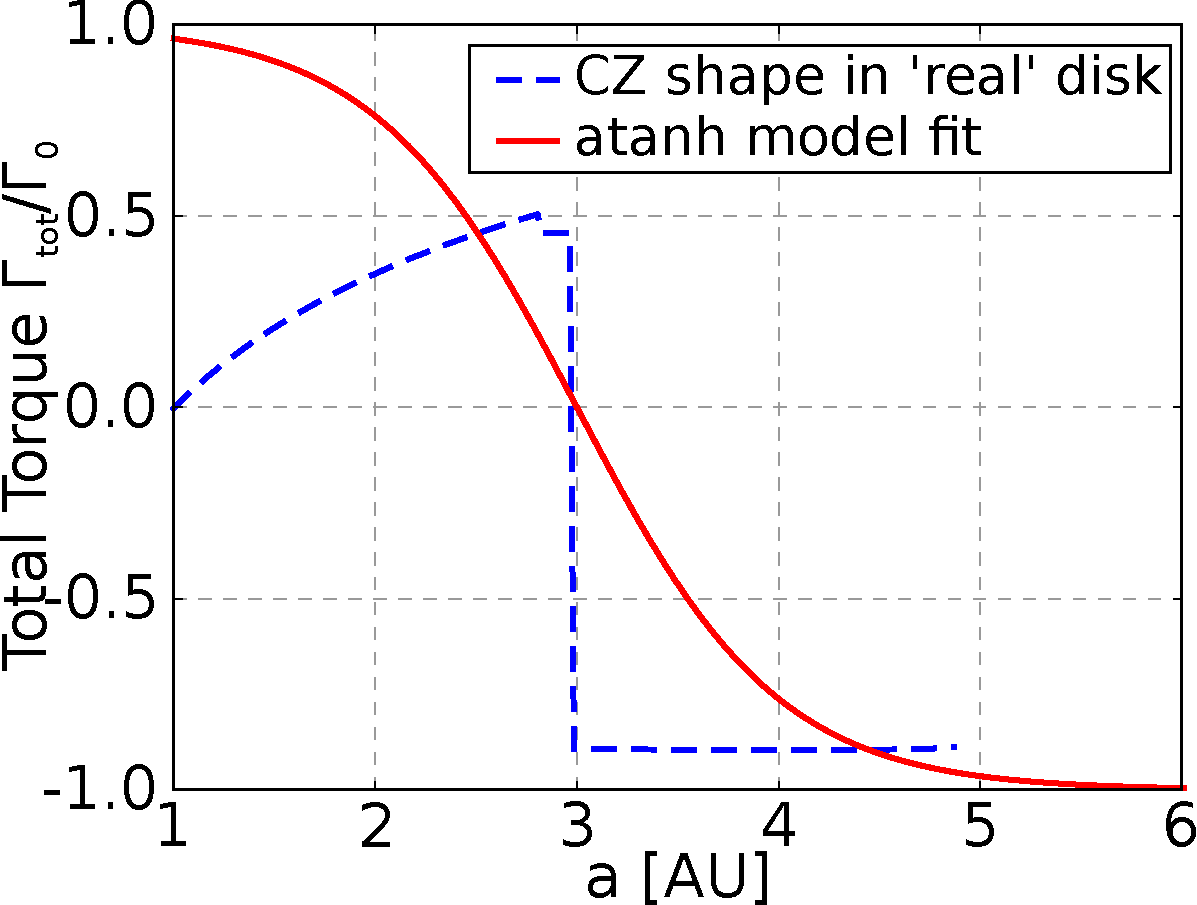
\includegraphics[width=0.49\linewidth]{figure/shifted/torque_zoom_CZ1.pdf}
\caption{Le couple total de notre disque standard est représenté en rouge. La ligne bleue pointillée représente le profil de couple ressenti par une planète de $10\unit{M_\oplus}$ autour d'une transition d'opacité, calculé à partir des équations de \cite{paardekooper2011torque}.}\label{fig:shifted_CZ_torque_prof}
\end{figure}

À noter qu'une fonction de Heavyside n'a pas été utilisée car la marche d'escalier dans le profil \textit{réel} n'est due qu'au fait que la table d'opacité n'a pas été lissée. On s'attend à ce que la transition soit plus douce dans la réalité.
%TODO arnaud veut que je compare une version lissée avec mon tangente hyperbolique.

La position de la zone de convergence était $3\unit{UA}$. À l'intérieur de $3\unit{UA}$, le couple est positif et égal à $\Gamma_0 = \left(\frac{q}{h}\right)^2\Sigma_p {r_p}^4 {\Omega_p}^2$., la migration se fait donc vers l'extérieur. Au delà de $3\unit{UA}$, le couple total est égal à $-\Gamma_0$. Ici $q$ est le rapport entre les masses de la planète et de l'étoile, $h$ est le rapport d'aspect qui dépend du profil de température mais vaut typiquement $0.05$. $\Sigma_p$, $r_p$ et $\Omega_p$ sont respectivement la densité de surface, la distance orbitale et la vitesse angulaire pour la planète. 

Le couple total est la somme du couple différentiel de Lindblad $\Gamma_L$ --- que l'on suppose constant et indépendant de $e$ --- et le couple de corotation $\Gamma_C$. Le principal intérêt de la zone de convergence artificielle est de s'affranchir de la forme très complexe du profil réel et ne garder que la zone de convergence, afin d'en étudier les effets de manière isolée.

\bigskip

\cite{bitsch2010orbital} montrent que la structure de la zone fer-à-cheval est modifiée quand l'excentricité augmente. En conséquence, son couple de corotation $\Gamma_C$, lié à cette région du disque, diminue. 

Nous avons élaboré une formule simple qui reproduit l'effet de l'excentricité sur $\Gamma_C$ par une simple calibration des simulations 3D de \cite{bitsch2010orbital} : 
\begin{align}
D &= \frac{\Gamma_C(e)}{\Gamma_C (e=0)} = 1 + a \cdot \left[\tanh(c) - \tanh\left(\frac{b * e}{x_s}+c\right)\right]\label{eq:shifted-eccentricity-influence}
\end{align}
où $x_s$ représente la demi-largeur de la région fer-à-cheval en unité de distance orbitale de la planète considérée, $e$ est l'excentricité de la planète, et notre ajustement statistique donne les valeurs suivantes pour les paramètres de la fonction :
\begin{align}
a &= 0.45 & b &= 3.46 & c &= -2.34
\end{align}

On défini $x_s$ comme \citep[eq. (44)]{paardekooper2010torque} :
\begin{align}
x_s &= \frac{1.1}{\gamma^{1/4}} \left(\frac{0.4}{b/h}\right)^{1/4} \sqrt{\frac{q}{h}}
\end{align}
où $\gamma$ est l'indice adiabatique, $q$ le rapport entre les masses de la planète et de l'étoile, $h$ le rapport d'aspect et $b/h$ la longueur de lissage du potentiel gravitationnel de la planète (dépendance issue des formules de \cite{paardekooper2011torque}).
%TODO c'est pas uniquement un problème numérique, c'est aussi un problème physique. Voir pour cela paardekooper et papaloizou 2009 ou encore kley & muller 2012
%TODO en gros, de ce que je comprends, il y a le problème de la masse ponctuelle de la planète qui génère une divergence quand on veut calculer la forme des ondes de densité générées par la planète sur le disque. Mais il y a aussi le problème de la longueur de lissage du potentiel du disque quand on veut calculer le couple du disque sur la planète. Il y a donc techniquement deux longueurs de lissages différentes. On doit choisir une seule longueur de lissage pour le potentiel gravitationnel, mais il y a deux longueurs de lissages "optimisées" si on veut faire le calcul d'audrey, JM ou arnaud proprement ; prescription de la longueur de lissage)

\reffig{fig:shifted_CZ_D_profile} montre que notre formule simple \refeq{eq:shifted-eccentricity-influence} correspond bien à la tendance des simulations hydrodynamiques de l'effet de $e$ sur $\Gamma_C$, en particulier pour les excentricités faibles. Il faut tout de même noter qu'il y a peu de points \og expérimentaux\fg et qu'il semble y avoir des fluctuations aléatoires influençant les valeurs mesurées.

\begin{figure}[htbp]
\centering
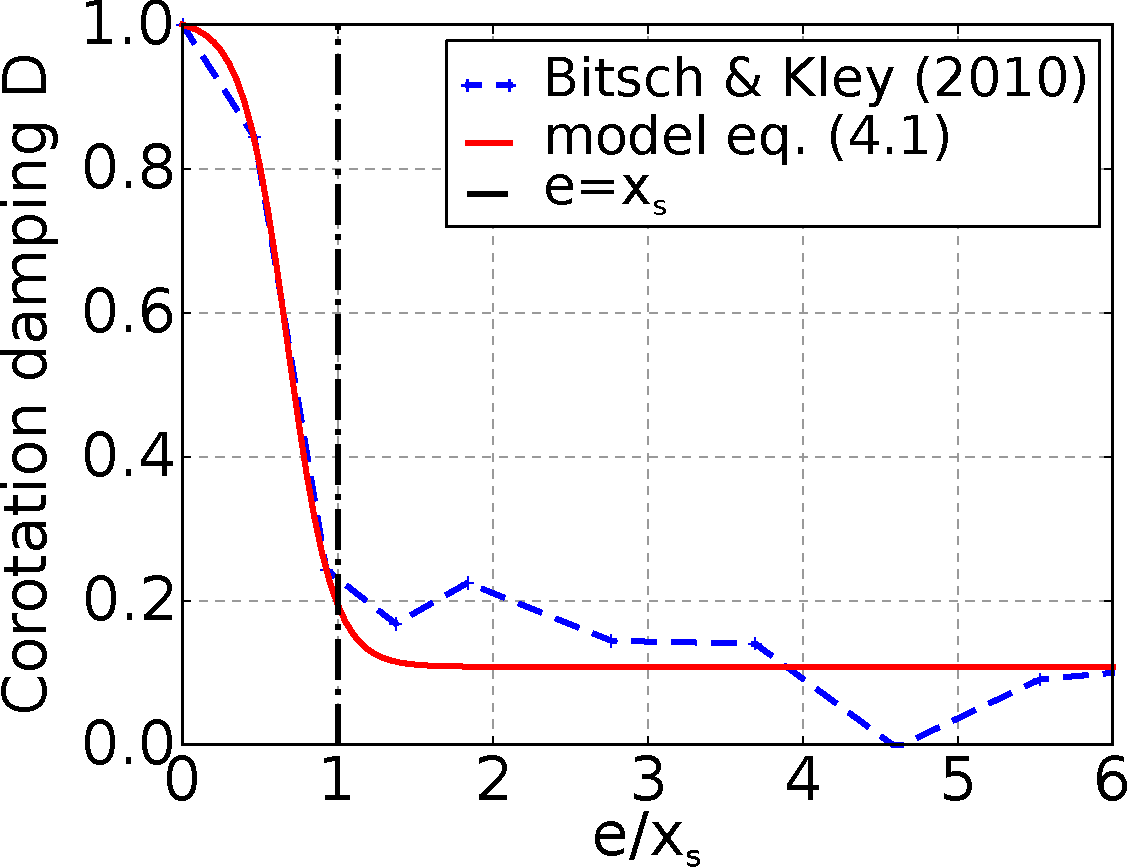
\includegraphics[width=0.49\linewidth]{figure/shifted/corotation_damping_profile.pdf}
\caption{Diminution du couple de corotation $\Gamma_C$ en fonction de l'excentricité $e$. On suppose que l'atténuation ($0<D<1$) du couple de corotation en fonction de l'extencité $e$ est la même dans un disque isotherme ou radiatif. Ainsi, on extrait la valeur de $D$ à partir de la figure 2 de \cite{bitsch2010orbital} en faisant la différence entre la valeur pour le disque radiatif et celle pour le disque isotherme, et normalisant de sorte que $D$ vale $1$ dans le cas $e=0$.}\label{fig:shifted_CZ_D_profile}
\end{figure}

\bigskip

Afin de réaliser nos simulations, nous avons utilisé la version modifiée de l'intégrateur \textbf{Mercury}\citep{chambers1999hybrid} décrite \refsec{sec:code_n-corps}. Nous avons utilisé en particulier la zone de convergence artificielle décrite \reffig{fig:shifted_CZ_torque_prof}. 

Nous supposons que le disque possède le profil de densité de surface suivant :
\begin{align}
\Sigma(R) = 500 \left(R/1\unit{AU}\right)^{-1/2} \unit{g.cm^{-2}}
\end{align}
Ce profil est alors utilisé dans le calcul de $\Gamma_0$ et de l'amortissement induit par le disque sur $e$ et $I$.

Pour implémenter la migration induite par le couple du disque $\Gamma$, on note que $\Gamma=\od{J}{t}$, et on défini une accélération de migration $a_m$ telle que\citep[eq. (14)]{cresswell2008three} :
\begin{align}
a_m &= - \frac{v}{t_m}
\end{align}
où $v$ est la vitesse de la planète et $t_m=J/\od{J}{t}$ le temps de migration ($J$ est le moment cinétique).

\bigskip

Dans toutes les simulations, les planètes était initialement sur des orbites à faible excentricité ($e<0.001$) et faible inclinaison ($I<1^\circ$). Chaque simulation a été intégrée pendant trois millions d'années, avec un pas de temps compris entre $0.4$ et $3$ jours.

\subsection{Le cas de deux planètes}
\reffig{fig:two-planets} montre l'évolution de deux planètes de $1\unit{M_\oplus}$ initialement placées de part et d'autre d'une zone de convergence située à $3\unit{UA}$. Alors qu'elles se rapprochent l'une de l'autre, les deux planètes croisent une série de résonances and finissent piégées dans la résonance \MMR{7}{6}. Les excentricités des deux planètes atteignent alors un équilibre entre excitation résonante et amortissement par le disque. Cette excentricité d'équilibre est environ égale à $0.5$ fois la demi-largeur de la zone fer-à-cheval $x_s$ et amortit le couple de corotation à environ $80\%$ de sa valeur nominale (quand $e=0$). 

\begin{figure}[htbp]
\centering
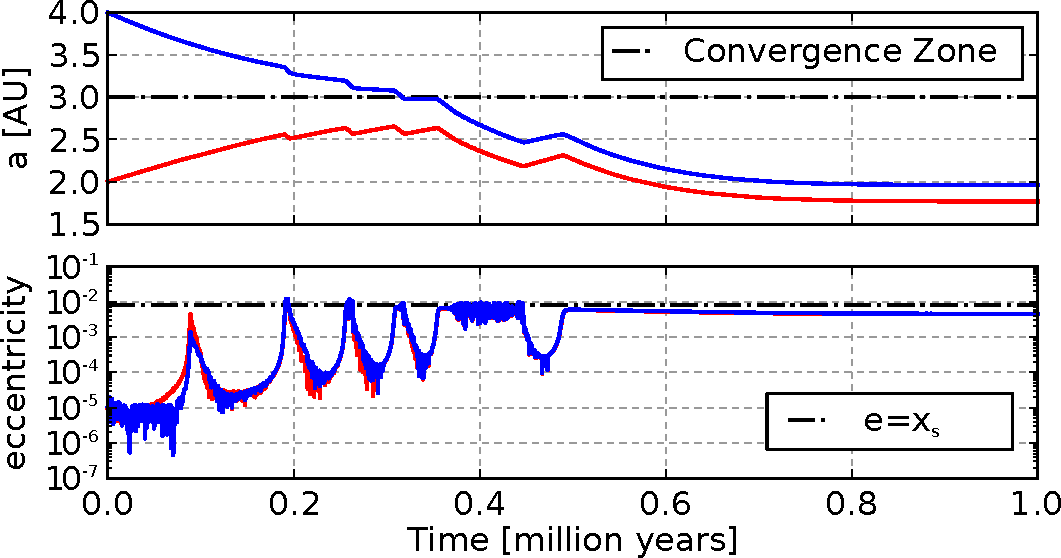
\includegraphics[width=\linewidth]{figure/shifted/corotation_damping_influence.pdf}
\caption{Simulation de la migration convergence de deux planètes de $1\unit{M_\oplus}$ vers la zone de convergence située à $3\unit{UA}$, la rétroactio de l'excentricité $e$ sur le couple de corotation $\Gamma_C$ étant incluse (voir Figure~\ref{fig:shifted_CZ_D_profile}).}
\label{fig:two-planets}
\end{figure}

Les planètes se stabilisent et arrêtent de migrer à $1.77$ et $1.96\unit{UA}$, toutes les deux à l'intérieur de la position nominale de la zone de convergence. Compte tenu de leurs excentricités, la zone de convergence de la planète la plus interne est décalée à $1.95\unit{UA}$ tandis qu'elle est décalée à $1.74\unit{UA}$ pour la planète externe (située à $1.96\unit{UA}$). On constate alors qu'aucune des deux planètes n'est à une position d'équilibre. Chacune d'elle ressent un couple dirigé vers l'autre planète du système, de sorte que la migration tend à rapprocher les planètes tandis que les résonances les maintiennent éloignées.

Le décalage de la zone d'équilibre provient ici de l'équilibre nouveau entre le couple de Lindblad resté inchangé et le couple de corotation atténué par l'excentricité. \emph{Les deux planètes se stabilisent autour d'une zone où le couple total exercé sur le système dans sa globalité est nul, même si chaque planète prise séparément ressent un couple de migration non nul}. Aucune des deux planètes n'est ici à une zone de convergence (même celle calculée en tenant compte de l'atténuation du couple de corotation). 

Il est clair que les excentricités des planètes --- excitées par les interactions entre planètes --- sont le facteur clé pour déterminer la force du couple de corotation et la position effective de la zone de stabilisation du système. Pour deux planètes de même masse, le même comportement qualitatif est observé, quelle que soit la masse ou la résonance considérée : Une plus grande excentricité implique un amortissement plus fort du couple de corotation $\Gamma_C$ et une stabilisation du système de plus en plus proche de leur étoile. 

\subsection{Effet du rapport de masse}\label{sec:mass-ratio-effect}
Nous étudions maintenant le cas de deux planètes de masses différentes. \reffig{fig:mass_ratio_final_pos} représente les positions finales d'une série de simulations simples dans lesquelles une planète de $10\unit{M_\oplus}$ est placée systématiquement à $3\unit{UA}$ en compagnie d'une autre planète, placée à $4\unit{UA}$ et dont la masse varie successivement entre $0.1$ et $3\unit{M_\oplus}$. 

\begin{figure}[htbp]
\centering
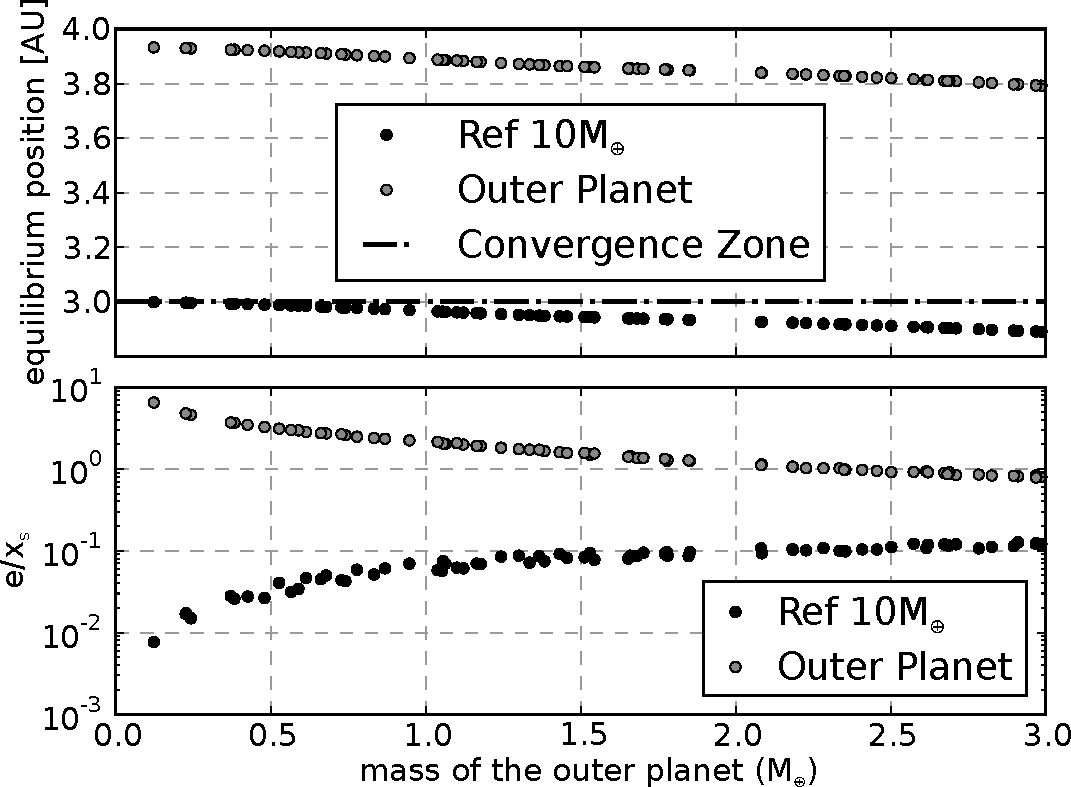
\includegraphics[width=0.95\linewidth]{figure/shifted/mass_ratio_influence.pdf}
\caption{Système final d'une série de simulations avec initialement une première planète à $3\unit{UA}$ de $10\unit{M_\oplus}$ et une deuxième planète à $4\unit{UA}$ dont la masse varie de $0.1$ à $3\unit{M_\oplus}$. Les graphiques montrent la position d'équilibre des planètes (en haut) et les excentricités normalisées par rapport à la demi-largeur de la zone fer-à-cheval $e/x_s$ (en bas) en fonction de la masse de la deuxième planète.}\label{fig:mass_ratio_final_pos}
\end{figure}

\bigskip

Dans \reffig{fig:mass_ratio_final_pos}, la planète externe est systématiquement en résonance \MMR{3}{2} avec la planète interne. Ainsi, la position finale des planètes est déterminée par leur masse respective ou, pour cette expérience, par la masse de la planète externe vu que la masse de la planète interne est fixe. 

Plus la deuxième planète est massive, et plus le décalage du système planétaire par rapport à la zone de convergence est important. En effet, une planète externe plus massive induit une excentricité plus importante pour la planète interne, ce qui correspond à un amortissement plus important de son couple de corotation $\Gamma_C$ et un décalage plus important de la zone d'équilibre du système. Compte tenu du fait que chaque planète possède une masse et une excentricité différentes, elles ressentent une zone de convergence différente (une pour chaque valeur de $e/x_s$). Pour autant, l'importance du décalage vers l'étoile centrale de la position d'équilibre est principalement déterminée par la dynamique de la planète la plus massive et de sa nouvelle zone de convergence.

\bigskip

\reffig{fig:mass_ratio_final_pos} représente uniquement un sous-ensemble de toutes les simulations de cette expérience. Pour des masses plus importantes, les deux planètes étaient dans des résonances différentes, ce qui causait des discontinuités dans le diagramme, rendant difficile sa lecture. Malgré tout, le comportement du système de deux planètes est qualitativement le même.

\subsection{Effet des résonances}
Dans la position d'équilibre d'un système de deux planètes, le degré de la résonance entre les deux corps est aussi important (pour une résonance de moyen mouvement \MMR{(p+q)}{p}, $p$ est le degré, et $q$ l'ordre de la résonance). On ne considère ici que des résonances d'ordre 1 (\MMR{3}{2} ou \MMR{11}{10} par exemple).

Deux planètes en résonance \MMR{3}{2} auront des excentricités plus importantes que si elles étaient en résonance \MMR{11}{10}. L'explication simple est qu'une résonance de degré moins élevé implique des conjonctions plus fréquentes, et ainsi des perturbations plus importantes (voir \cite{murray2000solar} pour plus de détails). La résonance dans laquelle un système de deux planètes se place dépend de la vitesse de migration relative et du taux d'amortissement de l'excentricité par le disque (voir par exemple \cite{mustill2011general}). Ces deux derniers paramètres sont déterminés à la fois par le disque, le profil de couple et les positions initiales des planètes. 

\begin{figure}[htbp]
\centering
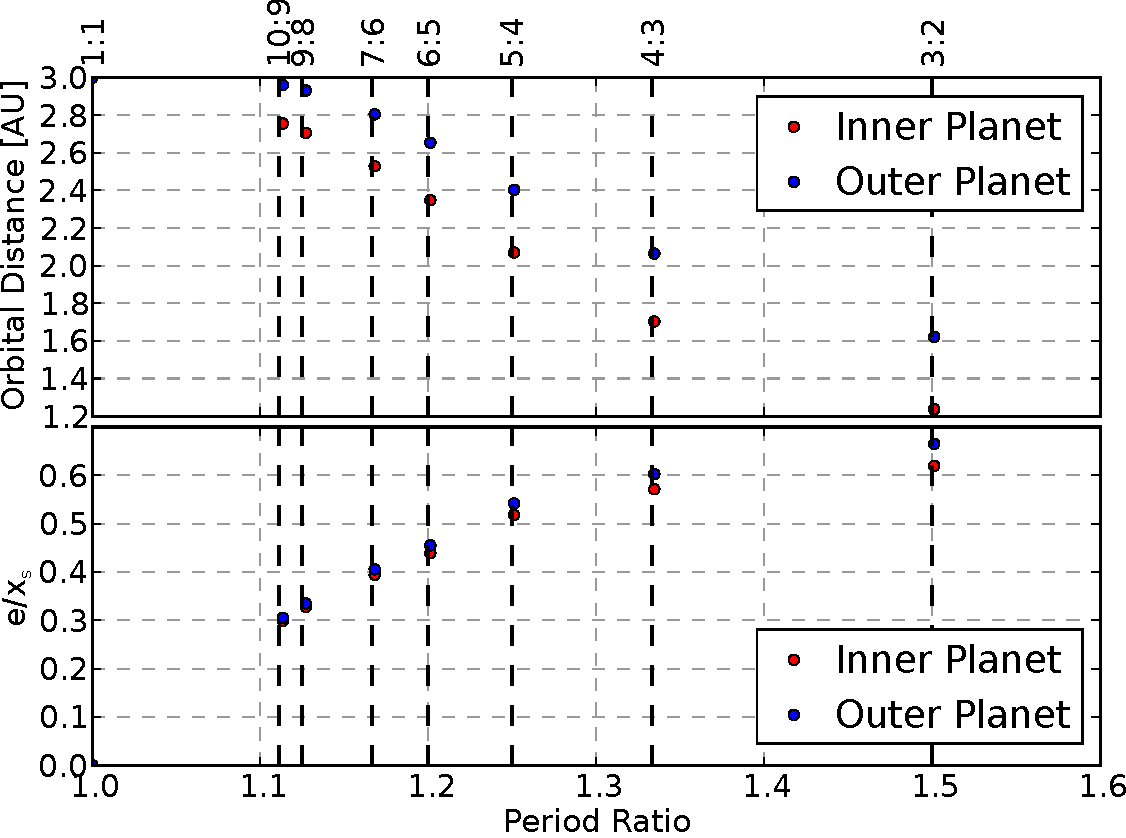
\includegraphics[width=0.95\linewidth]{figure/shifted/influence_of_MMR.pdf}
\caption{demi-grand axe final (en haut) et excentricité (en bas) de deux planètes de $3\unit{M_\oplus}$ piégées dans différentes résonances de moyen mouvement. Pour une planète de $3\unit{M_\oplus}$, la demi-largeur de la zone fer-à-cheval vaut environ $0.014$.}\label{fig:influence_of_MMR}
\end{figure}

Afin de tester l'effet des résonances, nous avons fait une série de 100 simulations (chacune intégrée pour un million d'années), avec deux planètes de $3\unit{M_\oplus}$ placés aléatoirement entre 1 et 10 UA, avec la même zone de convergence artificielle placée à 3 UA que précédemment. 

\reffig{fig:influence_of_MMR} montre que dans tous les cas, les planètes sont bloquées dans des résonances allant de \MMR{11}{10} à \MMR{3}{2} (degré de la résonance de 10 à 2). Conformément à ce qui était attendu, les excentricités maintenues grâce aux résonances diminuent à mesure que le degré des résonances augmente, et ceci induit un décalage moins important du système planétaire par rapport à la zone de convergence à 3 UA. L'amplitude du décalage vers l'intérieur de la position d'équilibre varie de 0.2 à 1.5 UA. 

Dans deux simulations, les planètes ont commencé si proches l'une de l'autre qu'elles se sont retrouvé en résonance co-orbitale (résonance \MMR{1}{1}). Dans ces cas là, leurs excentricités sont restées très faibles, et les deux planètes ont migré en co-orbite jusqu'à la zone de convergence nominale à 3 UA. 

\subsection{Évolution avec plus de deux planètes}
On se concentre maintenant sur le cas multi-planètes. Nous avons lancé 10 simulations pour des cas avec deux, trois, cinq ou dix planètes, initialement toutes de $3\unit{M_\oplus}$. Les planètes étaient placées aléatoirement entre 1 et 10 UA, et étaient sur des orbites de faible inclinaison et excentricité. Comme précédemment, chaque simulation a été intégrée pendant trois millions d'années dans un disque statique (sans dissipation). 

\bigskip

Dans les cas avec 3 planètes, on trouve 3 scénarii différents. Dans un premier cas, les 3 planètes sont prises dans une chaine de résonance et migrent vers l'intérieur toutes ensemble jusqu'à une zone d'équilibre où le couple total exercé sur le système est nul. Cette zone est typiquement entre 2 et 2.5 UA. Les excentricités des trois planètes ne sont pas identiques, la planète au centre de la chaîne de résonance est généralement la plus excitée. 

Dans le deuxième scénario le plus probable, deux planètes entrent en résonance et migrent vers l'intérieur tandis que la troisième et dernière planète est trop loin dans le disque pour être elle aussi prise en résonance avec les deux autres. Cette dernière planète migre alors à la zone de convergence à 3 UA, tandis que les deux planètes internes stoppent leur migration autour d'une zone d'équilibre où le couple total exercé sur le système est nul. 

Enfin, dans un troisième scénario, une collision a lieu et le système revient à un cas à deux planètes de masse différente comme vu précédemment \reffig{fig:mass_ratio_final_pos}. 

\bigskip

Pour les cas à 5 et 10 planètes, la situation est plus complexe. Les systèmes de 5 planètes forment des chaines de résonances et migrent vers l'intérieur, en direction d'une position d'équilibre où le couple total est nul. Cependant, les perturbations entre planètes ajoutent un aspect erratique à la migration des planètes. Même les systèmes les plus stables subissent des périodes d'instabilités durant lesquelles les planètes dérivent radialement dans la même direction. Ces périodes sont déclenchées par la sortie d'une résonance d'un couple de planètes à l'intérieur du système. Cette sortie de résonance se propage alors comme une perturbation à travers tout le système. L'amplitude et la fréquence de ces périodes chaotiques varient d'une simulation à l'autre. 

%\begin{figure}[htbp]
%\centering
%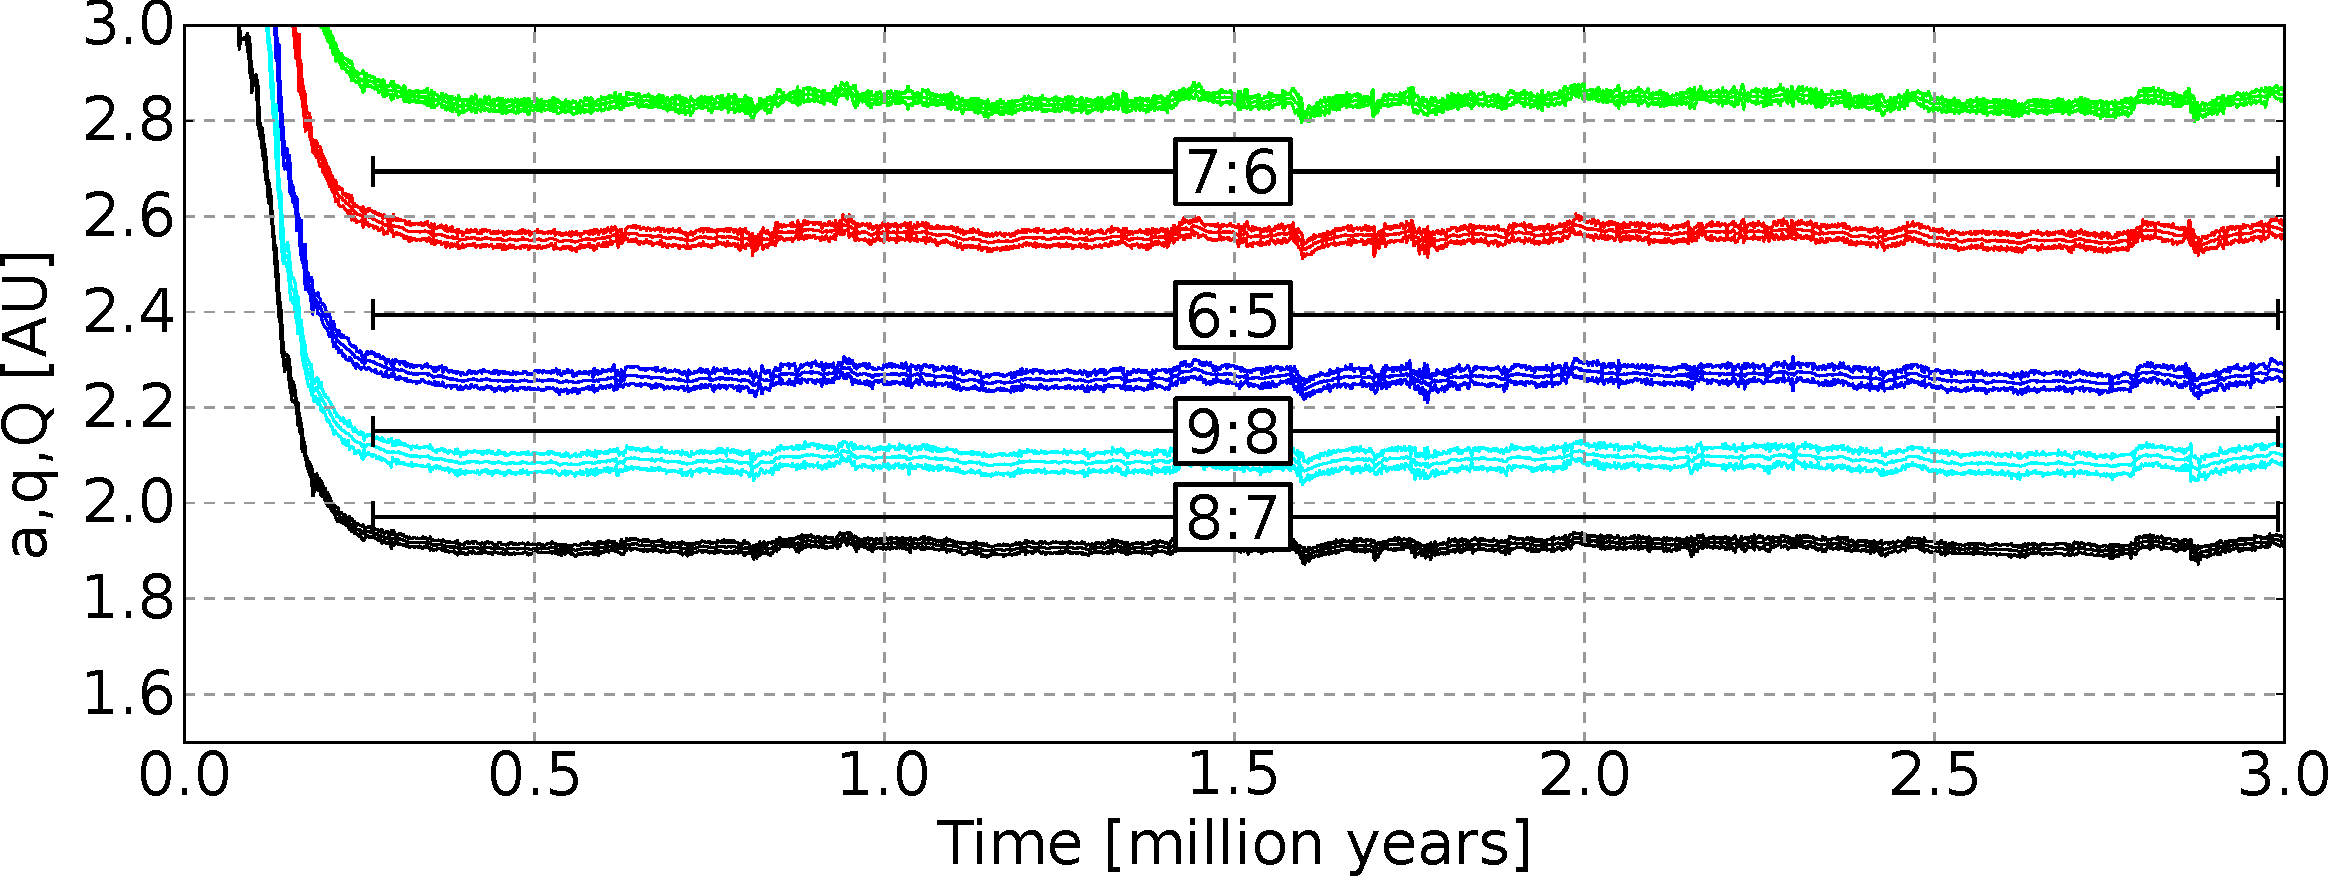
\includegraphics[width=\linewidth]{figure/shifted/5_simu00009_stable.pdf}\\
%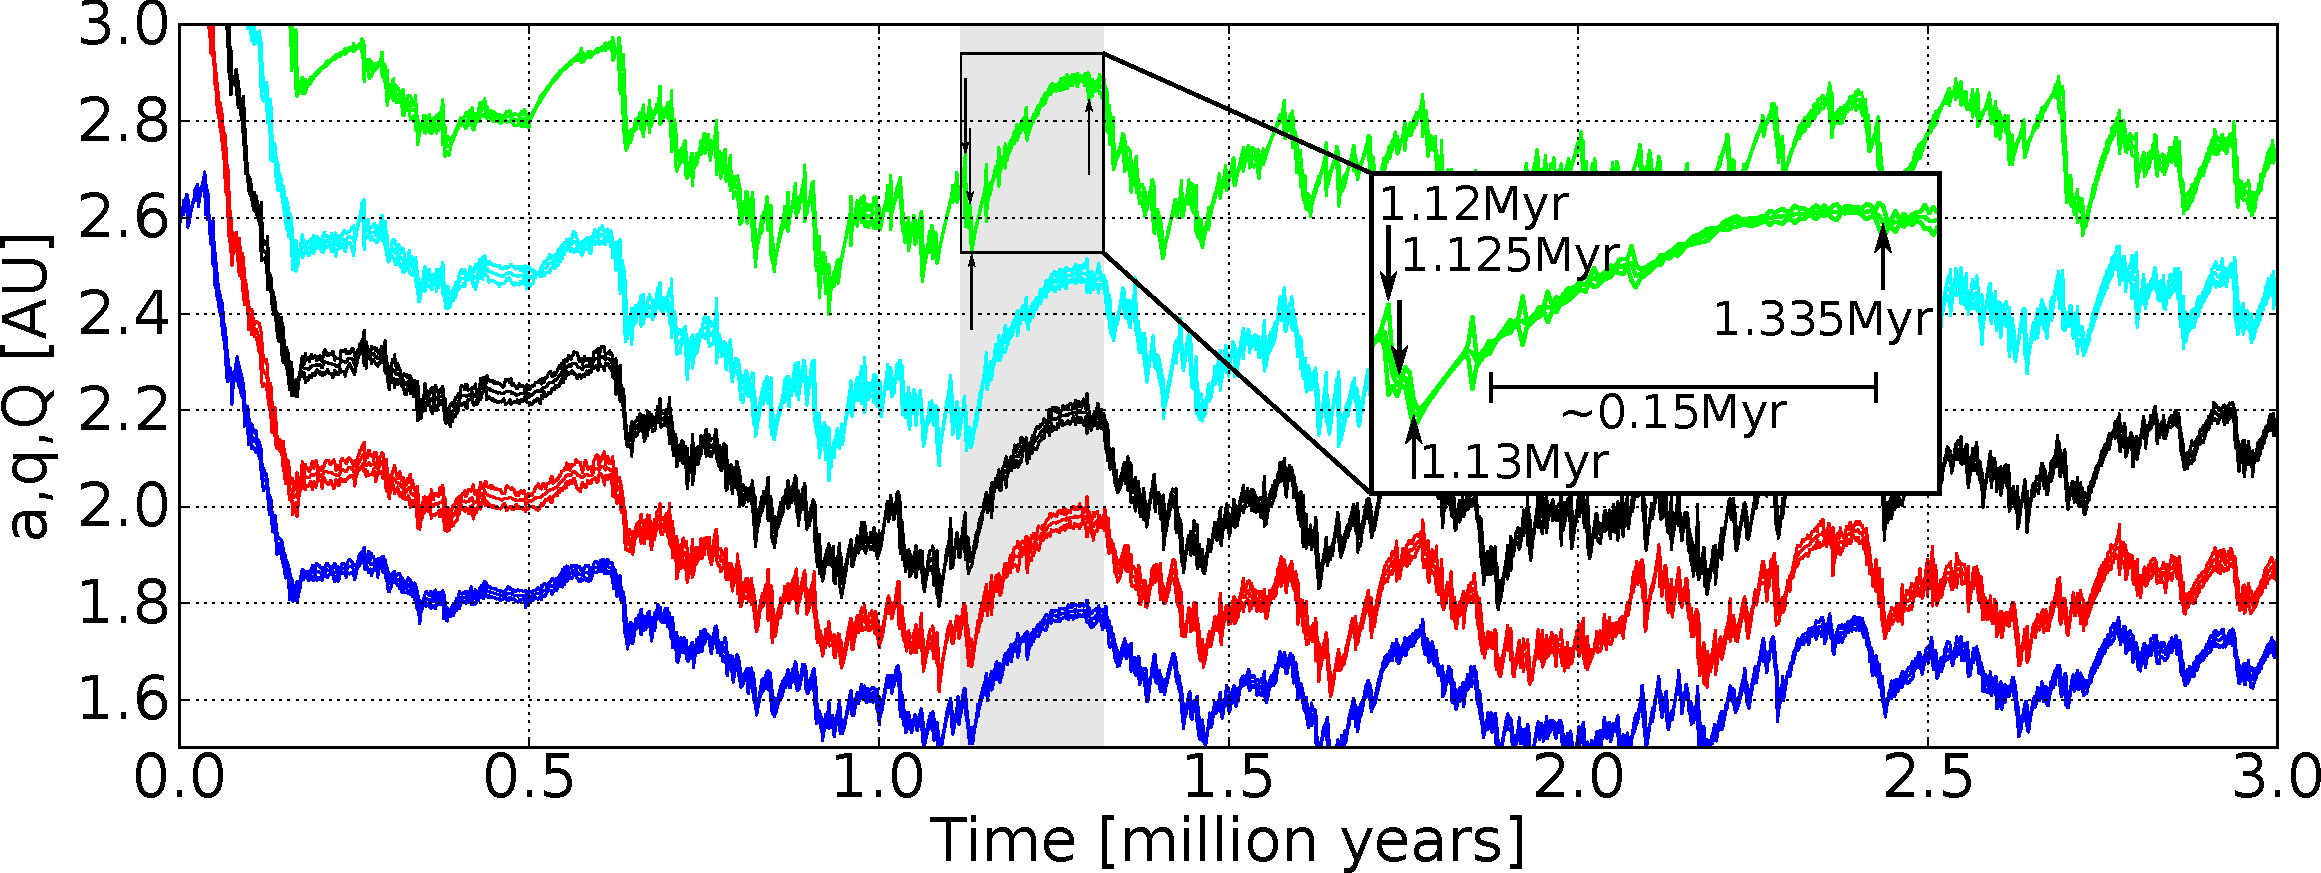
\includegraphics[width=\linewidth]{figure/shifted/5_simu00010_unstable.pdf}
%\caption{Deux exemples de simulations avec 5 planètes, une qui est relativement stable, même si de courts épisodes de pertubations des résonances ont lieu (en haut) et une qui possède un comportement chaotique soutenu (en bas).}
%\label{fig:timed-resonance-unstable}
%\end{figure}

\begin{figure}[htbp]
\centering
\subfloat[Simulation relativement stable, même si de courts épisodes de pertubations des résonances ont lieu]{\label{fig:timed-resonance-stable}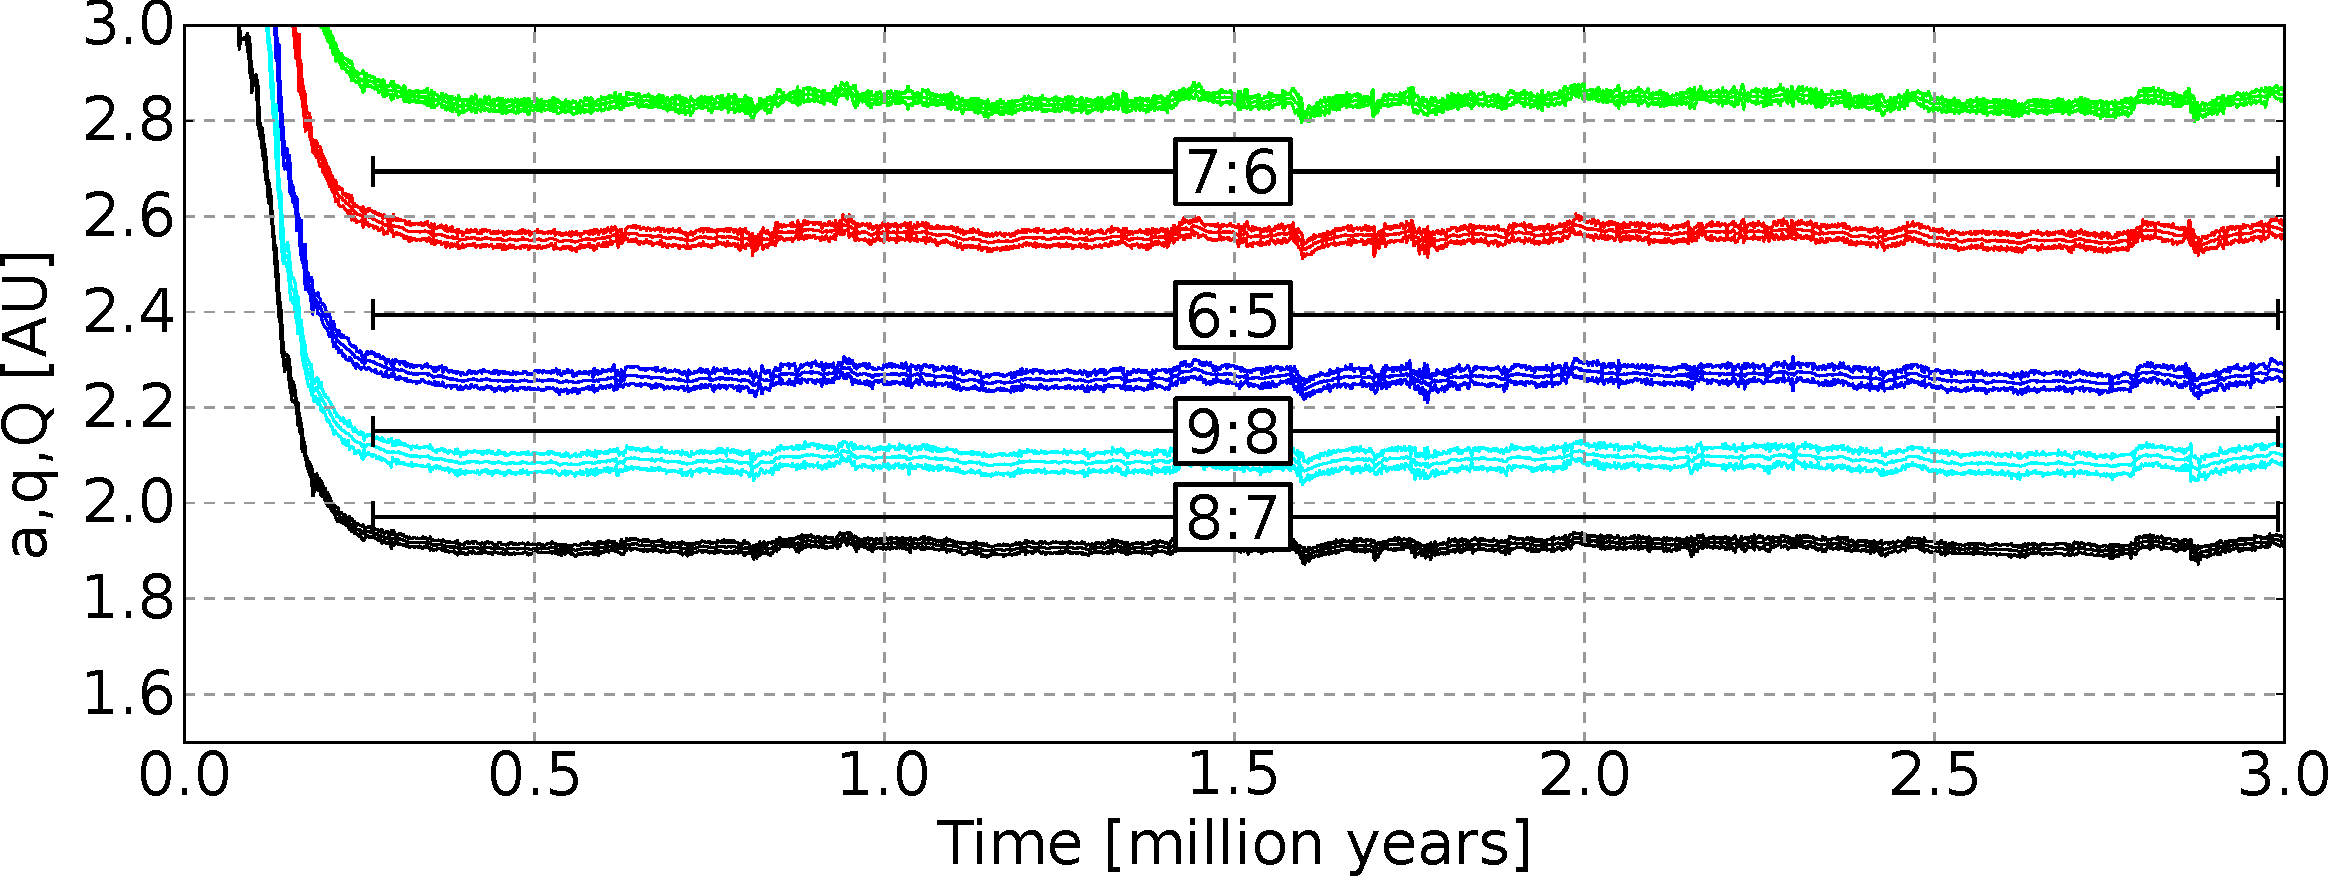
\includegraphics[width=\linewidth]{figure/shifted/5_simu00009_stable.pdf}}\\
\subfloat[Simulation qui possède un comportement chaotique soutenu]{\label{fig:timed-resonance-unstable}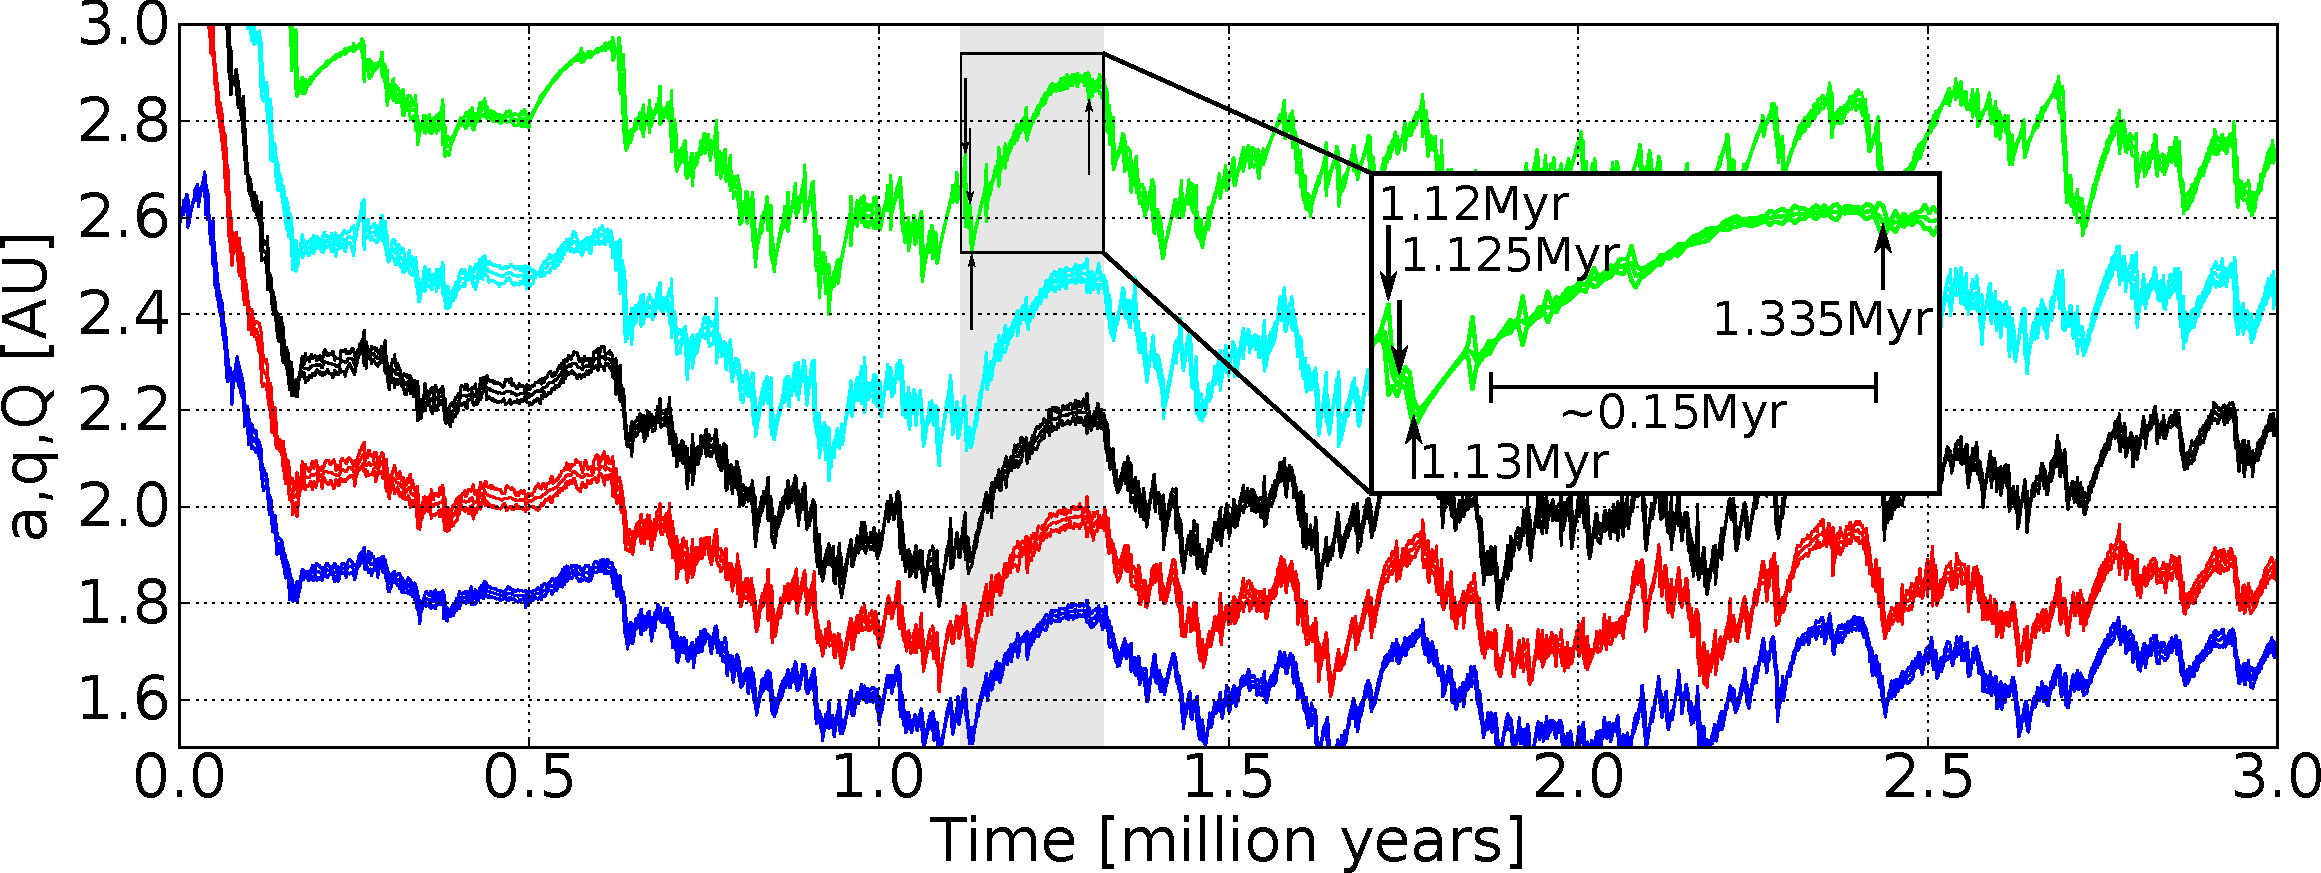
\includegraphics[width=\linewidth]{figure/shifted/5_simu00010_unstable.pdf}}
\caption{Deux exemples de simulations avec 5 planètes}\label{fig:timed-resonance-stability}
\end{figure}

Par exemple, dans la simulation \reffig{fig:timed-resonance-stable}, la chaine de  résonance subit plusieurs petites perturbations sans grandes conséquences car leur amplitude est faible devant la distance entre les planètes. Par opposition, les perturbations de la simulation  \reffig{fig:timed-resonance-unstable} sont bien plus importantes.

Considérons en particulier l'épisode chaotique entre 1.1 et 1.3 million d'années dans le cas décrit \reffig{fig:timed-resonance-unstable}. À 1.12 million d'années, les deux planètes externes sont piégées dans une résonance orbitale \MMR{4}{3}. Elles migrent alors vers l'intérieur, à cause de la soudaine excitation de leurs excentricités via la résonance. Cette perturbation se propage alors vers le système interne, et les excentricités de toutes les planètes augmentant soudainement, le système total se met peu à peu à migrer entièrement vers l'intérieur. 5000 ans plus tard, les deux planètes externes, encore les mêmes, sortent puis entrent de nouveau en résonance \MMR{4}{3}, perturbant de nouveau le système. Finalement, à 1.13 million d'années, les deux planètes externes sortent définitivement de la résonance \MMR{4}{3}. Retrouvant leur liberté de corps isolé, les deux planètes migrent vers la zone de convergence avec leurs excentricités de nouveau quasi nulle, la résonance n'étant plus là pour maintenir les 
excentricités face à l'amortissement du disque.

Sans le couple négatif des deux planètes externes, l'équilibre des couples du système global est modifié. En réaction, le système interne de trois planètes migre vers l'extérieur vers une nouvelle zone d'équilibre où le couple total exercé sur le système de trois planètes est nul. Ceci explique alors pourquoi les 5 planètes migrent brutalement vers l'extérieur. 

Cependant, les deux planètes externes entrent rapidement en résonance \MMR{5}{4}. Pendant les quelques 0.15 million d'années suivants, elles entrent périodiquement en résonance \MMR{5}{4} mais la migration vers l'extérieur continue car la plupart du temps elles ne sont pas en résonance et leur excentricité reste relativement faible. La migration globale vers l'extérieur du système s'arrête à 1.335 million d'années quand les deux planètes externes traversent la résonance \MMR{5}{4} et sont piégées dans la résonance orbitale \MMR{6}{5}. Cette configuration stabilise le système, excite les excentricités des planètes externes et entraine la migration globale du système tout entier vers l'intérieur, marquant la fin de cet épisode chaotique. 

\bigskip

Le reste de l'évolution est composé du même type de perturbations. Les perturbations proviennent des planètes qui entrent ou sortent des résonances, et qui se propagent alors au reste du système. 

Quand les planètes sortent de résonance, leur excentricité décroit rapidement, entrainant une migration vers l'extérieur. Par opposition, les planètes entrant en résonance voient leur excentricité croitre et être maintenue à un niveau constant non nul qui entraine une migration vers l'intérieur. 

Au travers de ces perturbations, des systèmes entiers subissent des migrations chaotiques relativement modestes qui illustrent la difficulté pour le système de maintenir une chaine de résonance pendant de longues périodes. 

La totalité des systèmes de 5 planètes que nous avons modélisés est restée stable, dans le sens où aucune collision n'a eu lieu. Mais l'amplitude de la migration chaotique subie par le système varie d'un système à l'autre. Les deux exemples de \reffig{fig:timed-resonance-stability} montrent les deux cas les plus extrêmes. Les simulations avec 10 planètes étaient encore plus chaotiques et des collisions ont eu lieu. 

\bigskip

Le point le plus important pour déterminer l'amplitude des oscillations chaotiques d'un système est le degré des résonances. Des résonances de degré $p$ faible (par exemple \MMR{3}{2}) maintiennent des excentricités élevés et sont moins stables car elles sont sensibles aux variations d'excentricité. Dans le même temps, les résonances de degré $p$ élevé (par exemple \MMR{11}{10}) maintiennent des excentricités plus faibles et sont moins sensibles aux perturbations d'excentricité.

Par exemple \reffig{fig:timed-resonance-stable}, les perturbations sont rapidement amorties tandis que dans le panneau du bas, la fréquence des perturbations est suffisamment importante pour que le système n'ait pas le temps de les amortir et ne tendent donc pas vers une configuration stable. \emph{Dans ce contexte, un système compact est donc plus stable qu'un système plus étendu, ce qui est exactement l'opposé d'une situation purement gravitationnelle} \citep{marchal1982hill}.

\subsection{Discussion}
Au travers de cette partie, nous avons montré que les planètes ne sont pas forcément piégées à la zone de convergence. Au lieu de cela, les embryons migrent rapidement vers la zone de convergence et sont piégés dans des chaînes de résonance. Ceci entraine l'augmentation brutale de leur excentricité qui reste suffisamment importante pour atténuer le couple de corotation. La zone d'équilibre de la chaîne de résonance dans le disque est déterminée par la somme des couples ressentis individuellement par les planètes (chaque terme étant la somme d'un couple de corotation atténué et d'un couple différentiel de Lindblad non atténué). Dans la pratique, cette zone de couple nul effective est déterminée principalement par la zone de convergence décalée de la planète la plus massive de la chaîne de résonance. Ce n'est pas une vraie zone de convergence car chaque planète voit une zone de convergence différente en fonction de son excentricité.

\bigskip

Le décalage vers l'intérieur existe parce que les excentricités des planètes sont maintenues par les perturbations résonantes. L'amplitude de l'excentricité d'une planète est le résultat de la compétition entre l'excitation résonante et l'amortissement de l'excentricité par le disque. Pour des excentricités suffisamment importantes, un système entier de planètes en résonance peut migrer jusqu'au bord interne.

Changer les propriétés du disque pourrait ainsi changer les valeurs typiques des excentricités en modifiant le temps caractéristique d'amortissement des excentricités. Cependant, changer les propriétés du disque a aussi des conséquences sur d'autres grandeurs influençant le système, tel que le profil de couple exercé par le disque sur les planètes. En changeant les propriétés du disque, il n'est pas évident de dire quelles seront les conséquences sur l'évolution des planètes, compte tenu du fait que les planètes pourront être dans des résonances différentes, avec des excentricités et des critères de stabilité différents. 

La zone de convergence dépend des paramètres du disque tels que la viscosité, les profils de température et de densité de surface \citep[voir par exemple][]{paardekooper2011torque}.Ici, nous avons utilisé un profil de disque issu de modèles complexes, mais qui reste malgré tout artificiel. Même si les résultats dépendent d'un modèle particulier, ils sont robustes aux variation du profil de couple en fonction de la distance orbitale, tant qu'une zone de convergence existe pour rassembler les embryons au cours de l'évolution. 

\bigskip

Dans un disque plus réaliste, on s'attend à quelques différences. En premier lieu, il pourrait exister plusieurs zones de convergence dans un même disque ayant pour origine des processus physiques différents \citep{lyra2010orbital, hasegawa2011origin}. 

Ensuite, des zones de convergences dépendantes de la masse des planètes peuvent exister dans les parties externes du disque, où ce mécanisme devrait être moins efficace compte tenu du fait que dans de telles zones de convergence, les embryons de masse différentes ne migrent pas à la même position dans le disque. Dans de telles zones, il pourrait être beaucoup plus difficile de former les chaînes de résonances essentielles pour notre mécanisme.

Troisièmement, alors que le disque se dissipe, le profil de couple et la position des zones de convergences sont aussi altérées \citep{lyra2010orbital, horn2012orbital}. 

Enfin, la turbulence est censée être commune dans les disques protoplanétaires \citep{armitage2011dynamics}. Même si la turbulence n'affecte pas l'évolution à long terme d'une planète isolée dans un disque radiatif \citep{pierens2012protoplanetary}, on s'attend à ce qu'elle modifie la capture en résonance et l'évolution des excentricités \citep[voir][]{pierens2011dynamics}.

\section{Formation des super-Terres chaudes}\label{sec:4.2}
Les détections d'exoplanètes par vitesse radiale et transit montrent que $30$ à $50\%$ des étoiles de la séquence principale possèdent au moins une planète de moins de $10\mearth$ sur des orbites comprises entre $85$ et $100$ jours \citep{mayor2011road, howard2010occurrence, howard2012occurrence, fressin2013false}. De plus, les super-Terres ($1-10\mearth$) chaudes sont préférentiellement détectées dans des systèmes multiples \citep{udry2007statistical, lissauer2011architecture}. Pourtant, même si ces systèmes peuvent nous sembler bien plus compacts que le système solaire au premier abord, d'un point de vue gravitationnel, ils possèdent à peu près le même espacement en terme de rapport de période et de rayon de Hill mutuel \citep{fang2013planetary}.


\reffig{fig:multiplanet_stats} montre les propriétés statistiques des planètes détectées dans des systèmes multiples, incluant les candidats Kepler.%TODO raconter plus de choses sur les stats?

\begin{figure}[htbp]
\centering
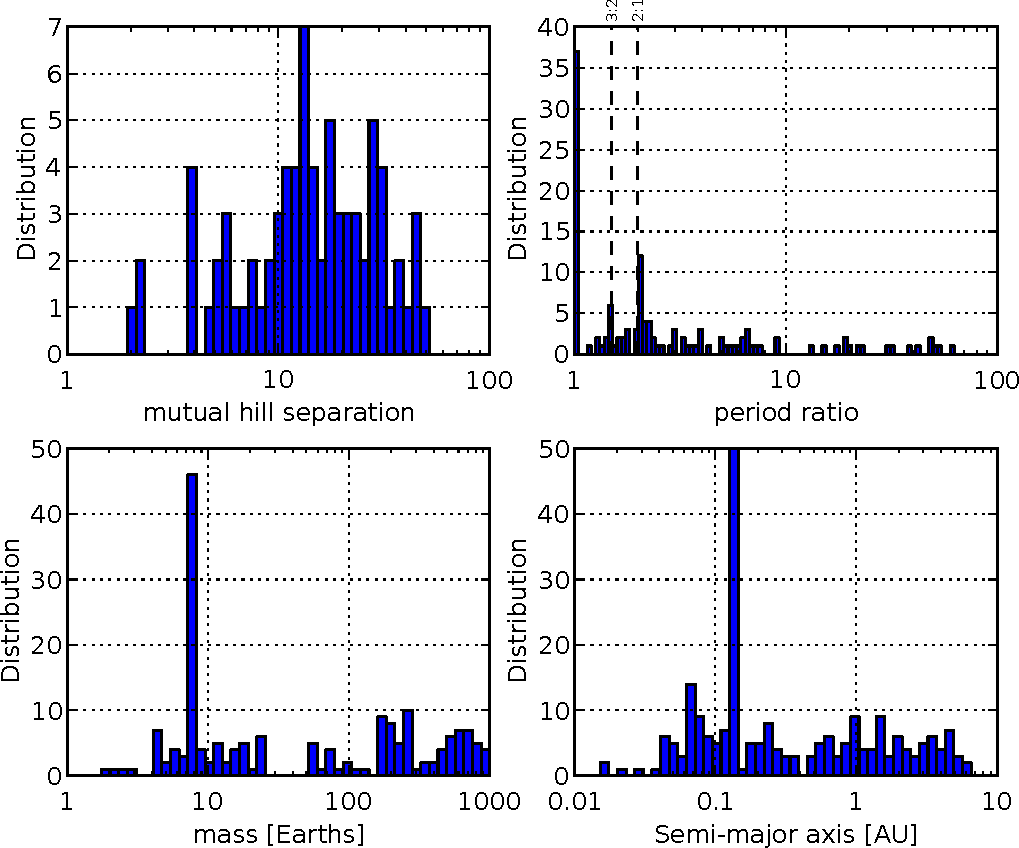
\includegraphics[width=0.8\linewidth]{figure/multiplanet_systems_stats.pdf}
\caption{Propriétés de toutes les exoplanètes détectées dans des systèmes multiples ($N\geqslant 2$). Données (01/01/2013) : \url{http://exoplanets.org/}}\label{fig:multiplanet_stats}
\end{figure}

\bigskip

Plusieurs mécanismes de formations tentent d'expliquer la présence de super Terres, ces planètes ayant une masse de $1$ à $10\mearth$, tout en étant compatible avec les contraintes observationnelles. Deux modèles principaux peuvent à ce jour expliquer la formation de ces planètes. 

Le premier modèle, la \og formation \textit{in-situ}\fg \citep{chiang2013minimum} n'est possible que si le disque est suffisamment massif localement pour permettre la formation de planète de plusieurs masses terrestres. Les dernières phases de la formation sont alors semblables à celles des planètes telluriques dans le système solaire \citep{wetherill1990formation, kenyon2006terrestrial}.

Le deuxième modèle implique la migration de type I \citep{terquem2007migration}. Dans ce cas là, il n'est pas nécessaire de supposer un disque extrêmement massif afin de former plusieurs super terres. 

Les deux modèles permettent d'expliquer l'espacement observé. Le modèle impliquant la migration de type 1 prédit aussi que les systèmes multiples vont être proches de résonances de moyen mouvement. On peut en effet observer des pics sur \reffig{fig:multiplanet_stats} autour des résonances \MMR{3}{2} et \MMR{2}{1}. Dans le cas de la formation \textit{in-situ}, on s'attend à des planètes assez pauvres en eau, alors qu'en impliquant la migration, la variété de composition des planètes ainsi formées est beaucoup plus grande \citep{raymond2008observable}.

Il existe de plus d'autres modèles, impliquant des résonances séculaires avec des planètes géantes plus loin dans le système, la photo-évaporation de super Neptunes, circularisation des planètes excentriques. Ces modèles sont présentés et comparés dans \cite{raymond2008observable} et ne sont pas discutés ici. 

%TODO 
%Observations : contraintes en fonction de la masse des planètes, séparation (en delta, et en p2/p1)
%
%autres modèles : 
%-in-situ (murray & hansens, ou chiang & laughlin, raymond 2008) il y a un résumé de tous les modèles dans raymond 2008
%-type I migraiton (terquem & papaloizou)
%
%_______
%environ une ou deux page pour cette intro

%TODO parler des raisons de la migration vers l'intérieur (intérieur car faible masse, ou intérieur car corotation damping). 
%TODO Parler aussi de ce qui arrête les planètes au bord interne. Faire des tests pour ça.

\subsection{Modèle}
Nous utilisons les formules de \cite{paardekooper2011torque} afin de modéliser la migration de type I. Cette migration est implémentée de manière cohérente dans tout le disque. Le bord interne est simplement modélisé par une diminution brutale de la densité de surface, mais le couple induit est lui toujours calculé selon les mêmes formules. 

L'amortissement de l'excentricité et de l'inclinaison est lui issu des formules de \cite{cresswell2008three}. 

Plus de détails sur le modèle utilisé sont disponibles \refsec{sec:code_n-corps}.

Le disque utilisé possède les paramètres suivants\footnote{voir \refsec{sec:variables} pour la signification des symboles usuels} : 
\begin{align*}
b/h &= 0.4\\
\gamma &= 7/5\\
\mu &= 2.35\\
\alpha &= 5\cdot 10^{-3}\\
T_\star &= 5700\unit{K}\\
R_\star &= 4.65\cdot 10^{-3}\unit{AU}\\
\text{Disk Albedo} &= 0.5\\
\Sigma(R) &= 300 \cdot R^{-1/2}\unit{g/cm^2}
\end{align*}

La migration d'une planète dans ce disque est représentée \reffig{fig:migration_map_HSE}. Ce graphique permet de visualiser les
zones de stabilités et l'évolution future d'une planète dans un disque en fonction de sa masse et de sa position initiale. Quand
le couple est positif, la planète migre vers l'extérieur (vers la droite du graphique). Quand le couple est négatif, la planète
migre vers l'intérieur (vers la gauche du graphique). Au cours de sa migration, si la planète rencontre une ligne noire, cela
signifie qu'elle s'arrête là, car le couple de migration est nul. Cette lecture n'est possible que pour des planètes isolées
dont l'excentricité est faible. En effet, les perturbations induites par d'autres planètes peuvent modifier l'état final prédit
par un tel diagramme, de même que l'amortissement du couple de corotation par l'excentricité d'une planète, qui va changer
le couple de migration ressenti par la planète. 

\begin{figure}[htbp]
\centering
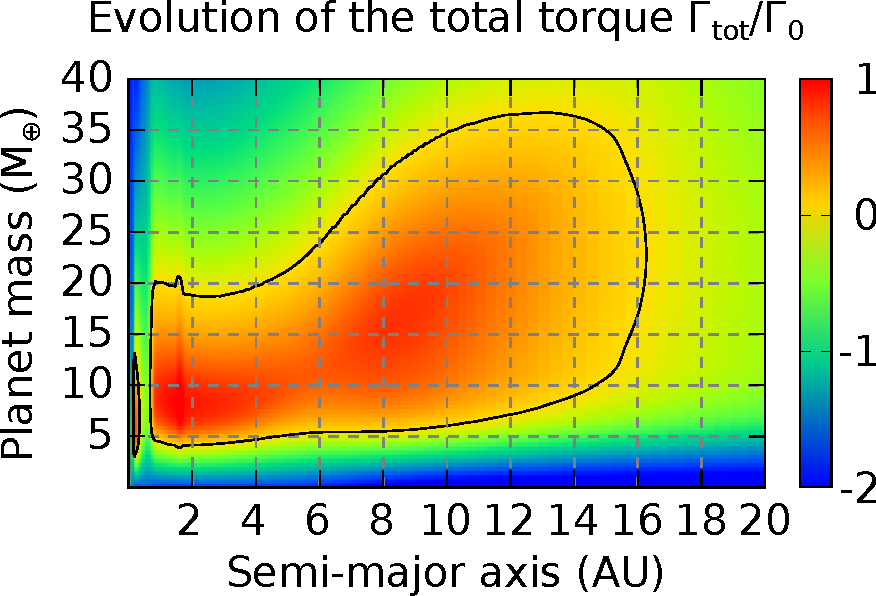
\includegraphics[width=0.65\linewidth]{figure/HSE/HSE_migration_map.pdf}
\caption{Cette carte représente l'effet du disque sur une planète en fonction de sa position en abscisse et de sa masse en ordonnée. La ligne noire représente la zone de couple nul, c'est à dire une zone où la migration de la planète s'arrête. Cette carte n'est valable que pour des planètes sur des orbites circulaires ($e\ll1$), c'est à dire quand l'amortissement du couple de corotation par l'excentricité est négligeable.}\label{fig:migration_map_HSE}
\end{figure}

Un zoom sur le bord interne du disque \reffig{fig:HSE_mig_zoom-in} montre la zone de couple positif juste avant le bord interne, dû à la décroissance rapide de la densité de surface et l'important couple de corotation qu'il engendre.

\begin{figure}[htbp]
\centering
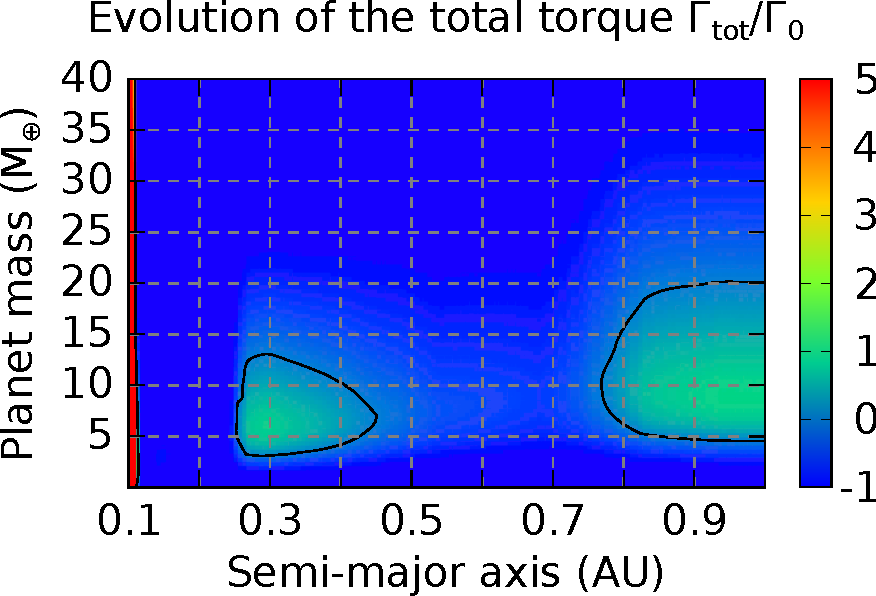
\includegraphics[width=0.65\linewidth]{figure/HSE/HSE_zoom-in.pdf}
\caption{Cette carte représente la migration d'une planète près du bord interne en fonction de sa position en abscisse et de sa masse en ordonnée. La ligne noire représente la zone de couple nul, c'est à dire une zone où la migration de la planète s'arrête. Cette carte n'est valable que pour des planètes sur des orbites circulaires ($e\ll1$), c'est à dire quand l'amortissement du couple de corotation par l'excentricité est négligeable.}\label{fig:HSE_mig_zoom-in}
\end{figure}

\subsection{Conditions initiales}
Les planètes sont sur des orbites quasi circulaires et coplanaires initialement. De plus, elles sont placées aléatoirement sur leur orbite dont l'orientation est elle aussi aléatoire.

Les positions des planètes sont choisies de manière aléatoire et uniforme entre $1$ et $20\unit{UA}$. Un court épisode d'instabilité et de collisions peut survenir dès le début des simulations dans le cas où deux planètes se trouvent extrêmement proches. Il résulte en la formation d'une planète légèrement plus massive que les autres. 

Initialement dans le système, on génère des embryons dont la masse varie de $0.1$ à $2\mearth$, pour une masse totale allant de $30$ à $100\mearth$. Des masses aléatoires différentes d'un embryon à l'autre permettent d'éviter les biais dûs aux masses égales. En effet, deux embryons de même masse migrent à la même vitesse, ce qui n'a aucune raison physique de se produire systématiquement dans un disque. Deux planètes migrant à la même vitesse ne peuvent pas entrer en collision, ou se placer en résonance, deux évènements cruciaux pour notre mécanisme de formation. 

De plus, quand deux corps sont en résonance, il y a un effet du rapport de masse sur les niveaux réciproques d'excentricité. Des masses égales maximisent les perturbations gravitationnelles de deux corps en résonance \refsec{sec:mass-ratio-effect}. Sinon, c'est le plus gros corps qui impose la stabilisation du système de deux corps, le corps moins massif étant piégé dans une zone où il ne pourrait pas rester sans la présence du compagnon. Le corps le plus massif est aussi celui qui a l'excentricité la plus faible. En s'écartant d'un système de deux planètes de masse égale, on diminue ainsi le décalage vers l'intérieur de la zone de stabilisation.

Les masses sont choisies de telle sorte que l'on puisse avoir un nombre relativement importante de planètes initialement (autour de 60) pour une masse planétaire totale n'excédant pas $60\mearth$. En effet, il est essentiel d'avoir un nombre important d'embryons afin de mettre en évidence l'effet des résonances et des perturbations gravitationnelles. 

\subsection{Systèmes possibles}
En dessous d'une certaine masse limite qui dépend des paramètres du disque mais qui se situe généralement entre $2$ et $10\mearth$, les planètes migrent toutes vers l'intérieur, quelle que soit leur position initiale dans le disque. Pour le disque considéré ici \reffig{fig:migration_map_HSE}, cette limite se situe environ à $4\mearth$.

L'évolution peut suivre deux cas de figures différents, mais non exclusifs.

Dans un premier cas, les embryons migrent vers l'intérieur et il n'y a pas suffisamment de collisions durant leur migration pour qu'ils puissent migrer vers l'extérieur à un quelconque moment. On se trouve alors dans le cas d'une formation au bord interne décrite \refsec{sec:inner_edge_formation}. 

Dans un deuxième cas, une ou plusieurs planètes grossissent suffisamment par collision pour ressentir un couple positif vers l'extérieur. Plusieurs sous-cas de figures sont alors possibles, décrits \refsec{sec:outward-case}.

\subsubsection{Formation au bord interne : systèmes compacts}\label{sec:inner_edge_formation}
Des embryons migrent vers l'intérieur, de manière isolée ou par vague de sous-systèmes en résonance.

En raison de la diminution rapide de la densité de surface près du bord interne, la planète ressent un fort couple positif principalement dû au couple de corotation \reffig{fig:HSE_mig_zoom-in}. 

Un système de planètes en résonance se forme alors, les planètes internes migrant vers l'extérieur, les planètes externes migrant elles vers l'intérieur. Ce système en résonance va naturellement chercher à s'équilibrer. Cet équilibre est dicté par le fait que chaque planète ressent un couple non nul, elle possède aussi une excentricité à cause des autres corps en résonance, et ce système compact est continuellement soumis à des perturbations d'autant plus importantes que le nombre de corps en résonance est grand. 

\begin{figure}[htbp]
\centering
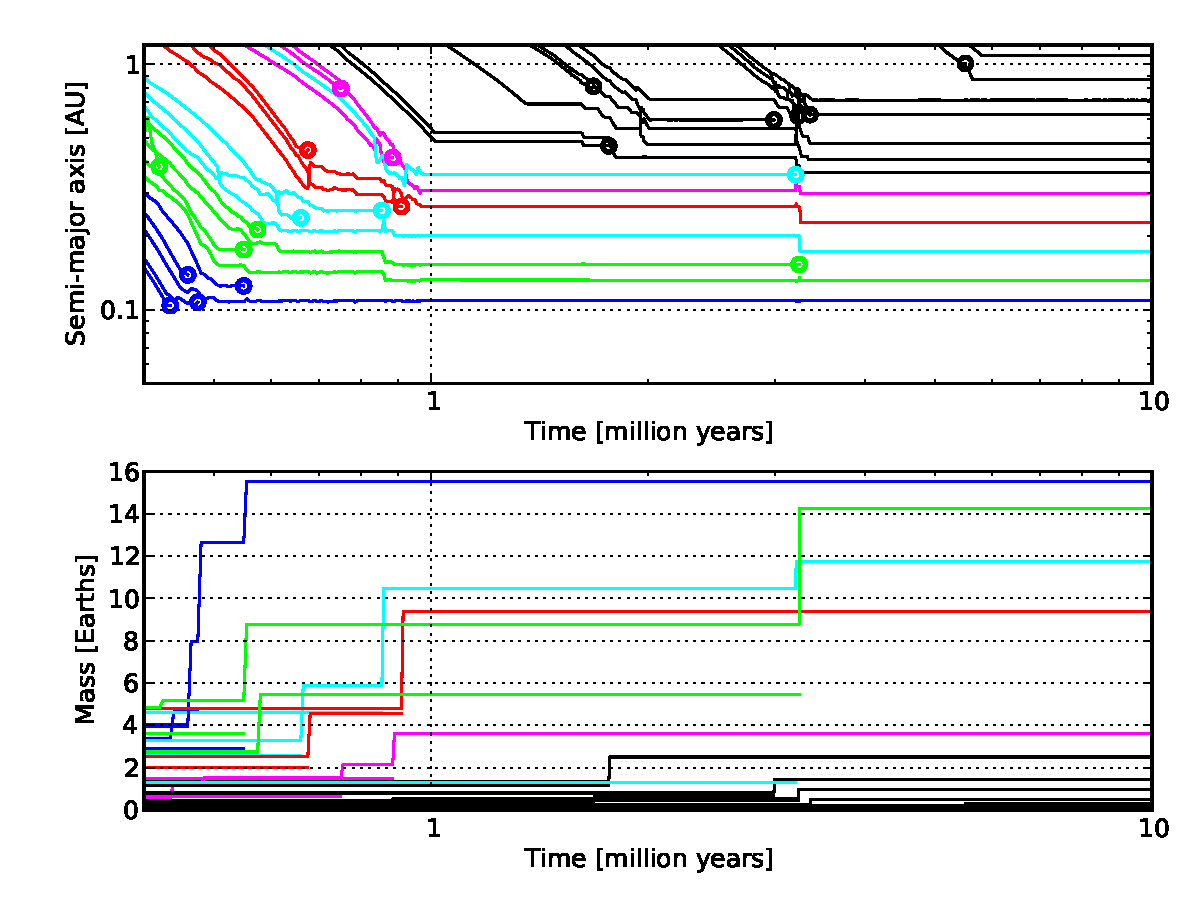
\includegraphics[width=0.7\linewidth]{figure/HSE/inner_system.pdf}
\caption{Zoom sur l'évolution des planètes près du bord interne du disque situé à $0.1\unit{UA}$. }\label{fig:HSE_inner_system}
\end{figure}

Des collisions et réarrangements ont alors lieu, diminuant ainsi le nombre de corps et augmentant la stabilité du système global \reffig{fig:HSE_inner_system}. Ces réarrangements peuvent en particulier être déclenchés par l'arrivée au bord interne d'une ou plusieurs planètes qui migraient moins rapidement que les autres. Par la compression supplémentaire qu'elles apportent au système, elles déclenchent des perturbations qui peuvent engendrer des collisions. C'est ce qu'il se produit sur  \reffig{fig:HSE_inner_system}, notamment à 3 millions d'années. 

\bigskip

Certaines planètes peuvent entrer dans la cavité interne du disque, poussées par le système non encore stabilisé. Elles ne perçoivent alors plus aucun effet du disque, que ce soit la migration ou l'amortissement de l'excentricité et de l'inclinaison. Dans ce cas de figure, elles peuvent ne plus être en résonance avec le reste du système. 

Même si durant l'évolution, il est possible que la planète la plus interne sorte du disque, entre en collision avec l'étoile centrale, ou soit ejectée, il est très facile de maintenir un système compact au bord interne en raison du fort couple positif qui va s'exercer sur le planète la plus interne du système alors que ce dernier cherche à migrer vers l'intérieur.

\subsubsection{Migration vers l'extérieur : candidats de planètes géantes}\label{sec:outward-case}
Lors de la migration vers l'intérieur de tous les embryons, il est possible pour une planète de grossir suffisamment vite pour ressentir un couple positif. Ce couple positif est censé entrainer une migration vers l'extérieur de la planète, ce serait systématiquement le cas si cette dernière était isolée. Mais dans son voisinage se trouvent d'autres planètes qui elles migrent vers l'intérieur. Très rapidement la planète va entrer en résonance avec un embryon planétaire qui migre vers l'intérieur.

L'effet décrit \refsec{sec:shifted_CZ} s'applique alors. La migration différentielle et le rapport de masse ont ici une importance capitale. Si la différence de vitesse est trop grande, alors les deux planètes ne peuvent pas former un système en résonance. La résonance est rapidement cassée et les deux corps continuent leur migration. Ceci est d'autant plus vrai si le rapport de masse est important, car la brève augmentation d'excentricité qui a lieu lors d'une capture en résonance n'aura que peu d'effet sur la plus grosse planète. Cette dernière sera très peu sensible aux perturbations gravitationnelle de son compagnon résonant et continuera sa migration vers l'extérieur sans quasiment ralentir. 

\begin{figure}[htbp]
\centering
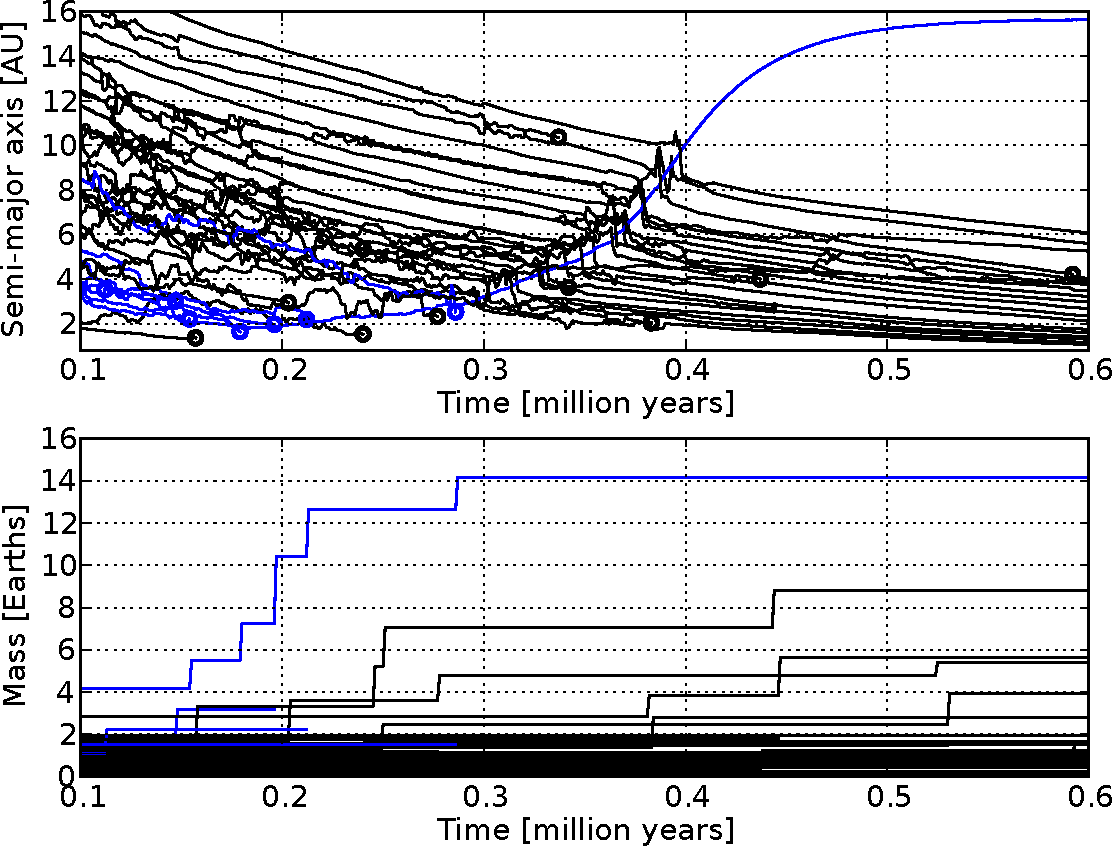
\includegraphics[width=0.65\linewidth]{figure/HSE/single_outward.pdf}
\caption{Formation d'un cœur de planète géante. La planète dont l'évolution est notée en bleu devient massive suffisamment vite pour pouvoir migrer vers l'extérieur. Les cercles représentent des collisions. Les autres courbes bleu qui disparaissent sont des embryons qui rentrent en collision avec la planète considérée et fusionnent avec elle. }\label{fig:single_outward}%/sse/cossou/HSE/disk_param/300_05/simu00010
\end{figure}

\reffig{fig:single_outward} illustre ce scénario. Cette dernière atteint par collisions la masse de $6\mearth$ au bout de $300 000\unit{ans}$ alors qu'elle se trouve à $1.2\unit{AU}$ ce qui est suffisant pour qu'elle puisse migrer vers l'extérieur. Cependant, les perturbations gravitationnelles des autres corps qui eux migrent vers l'intérieur l'empêchent de se comporter comme une planète isolée. Dans les quelques dizaines de milliers d'années suivants, 3 nouvelles collisions ont lieu. La planète fait maintenant $13\mearth$. La différence de masse avec ses voisins immédiats lui permet de migrer vers l'extérieur malgré les perturbations résonantes qui augmentent son excentricité. Comme détaillé \refsec{sec:mass-ratio-effect}, plus le rapport de masse est important, et plus la migration est dominée par la planète massive. Dans un système résonant avec rapport de masse élevé, la petite planète a une excentricité importante, son couple de corotation est fortement atténué, ce qui n'est pas le cas de la planète 
massive. Cette dernière migre comme si elle n'était pas en résonance, et à partir de là, soit elle emporte le système avec elle, soit, comme dans le cas présent, la résonance fini par se briser et les deux planètes continuent leur migration séparément.

Dans la suite de la simulation, la planète est trop massive pour être arrêtée. La planète massive migrant vers l'extérieur, elle capture en résonance un embryon de faible masse. Les deux planètes migrent alors vers l'extérieur, emportées par la migration de la planète la plus massive. Pourtant le système n'est pas stable. Les perturbations finissent par briser le système de deux planètes qui a alors deux possibilités. Soit une collision survient, augmentant sa masse, soit la brève rencontre se termine par un échange d'orbite. Dans cet exemple, les deux planètes continuent leur migration séparément.

À la fin de la simulation, la planète de $17.4\mearth$ est à sa zone de couple nul, à $15.7\unit{AU}$. 

\bigskip

Il est aussi possible pour la planète migrant vers l'extérieur de capturer en résonance une planète dans une configuration stable, comme le montre \reffig{fig:2-body_outward}.
\begin{figure}[htbp]
\centering
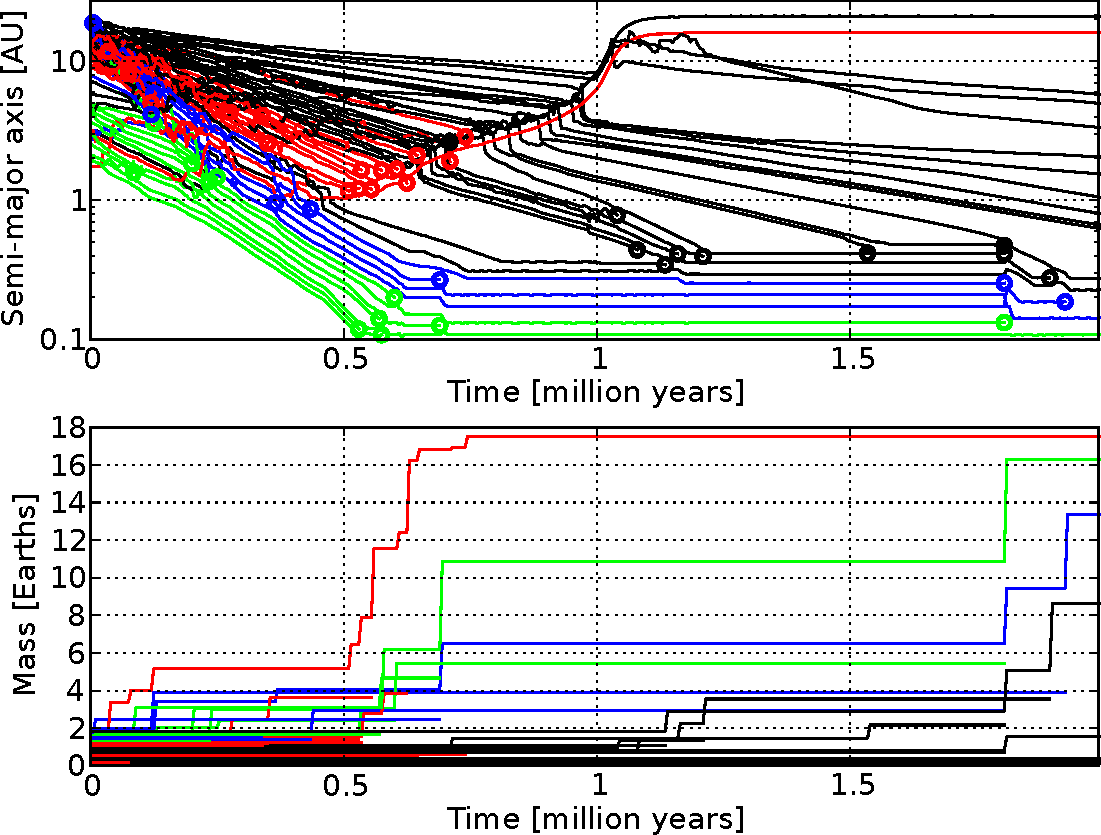
\includegraphics[width=0.65\linewidth]{figure/HSE/2-body_outward.pdf}
\caption{Formation d'un cœur de planète géante (en rouge) qui capture en résonance une planète de faible masse migrant très lentement vers l'intérieur.}\label{fig:2-body_outward}%/sse/cossou/HSE/disk_param/300_05/simu00038
\end{figure}

Dans cette même simulation, deux autres planètes massives sont formées (en vert et bleu) au bord interne, mais elles n'étaient pas massives suffisamment tôt pour migrer vers l'intérieur. Ainsi le même mécanisme, par un simple effet de timing, permet de créer soit des systèmes compacts de super terres chaudes, soit des embryons de planète géante qui pourront accréter du gaz dans les parties externes du disques, au delà de la ligne des glaces.

\bigskip

On a enfin un troisième et dernier cas où une planète grossit suffisamment rapidement pour migrer vers l'extérieur, mais est entrainée vers l'intérieur en étant capturée en résonance avec une planète ce qui inverse son sens de migration \reffig{fig:HSE_forced_in}. Dans ce système, la planète en rouge dans la figure ressent un couple de migration qui la pousse vers l'extérieur à partir de \nombre{229000} ans, quand une collision lui fait dépasser $5\mearth$. À ce stade, si elle avait été isolée dans le disque, elle aurait alors migrée vers l'extérieur jusqu'à se stabiliser autour de $9\unit{UA}$. Au lieu de cela, son excentricité reste élevée à cause des perturbations gravitationnelles des corps environnants. Son couple de migration est atténué jusqu'à que le sens en soit changé. La planète migre alors vers l'intérieur, entrainée par des résonances successives avec ses voisins. Même si les résonances changent, l'effet net est une migration vers l'intérieur car l'excentricité n'est jamais suffisamment amortie pour que la migration vers l'extérieur puisse s'effectuer.

\begin{figure}[htbp]
\centering
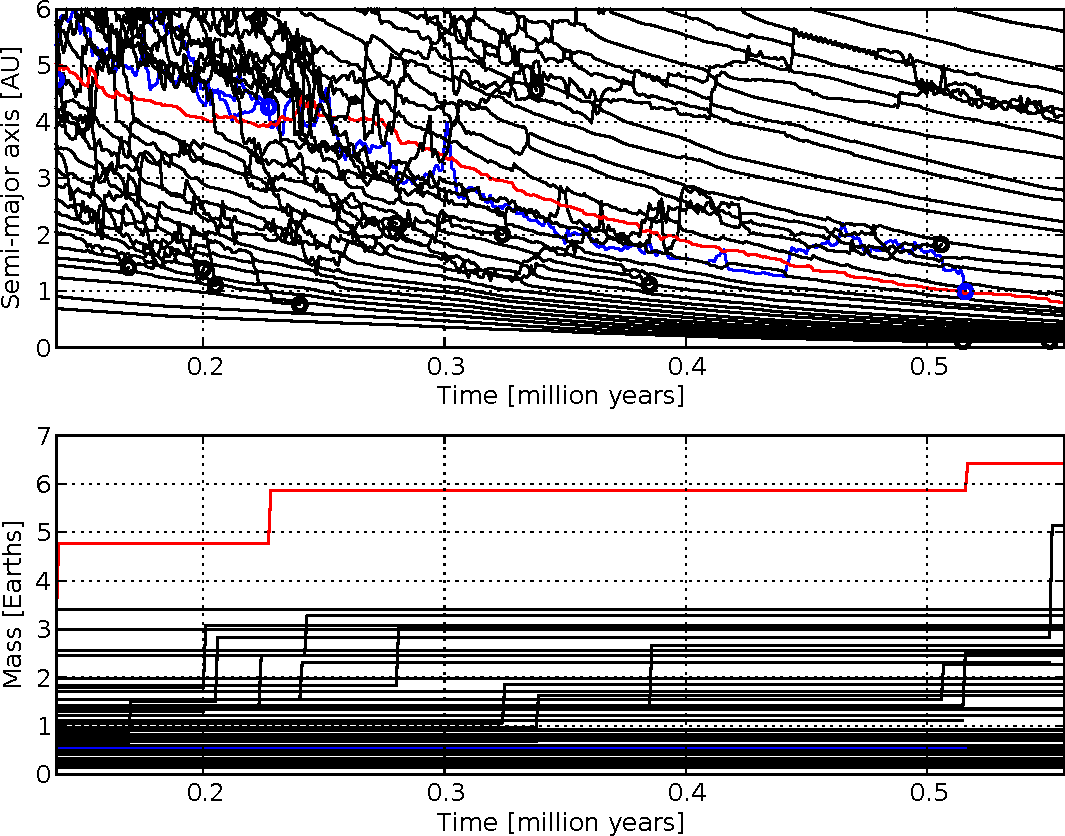
\includegraphics[width=0.65\linewidth]{figure/HSE/forced_in.pdf}
\caption{Migration forcée d'une planète (en rouge) vers l'intérieur par excitation de son excentricité. Les planètes en bleu rentrent en collision avec la planète qui nous intéresse (en rouge). La figure en bas montre l'évolution des masses au cours du temps. On remarque en particulier les deux collisions qui augmentent la masse de la planète rouge.}\label{fig:HSE_forced_in}
%/sse/cossou/phd/HSE_cond_inits/fiducials/simu00004
\end{figure}

%TODO regarder la simulation %/sse/cossou/HSE/disk_param/300_05/simu00001/hires pour celà

%TODO chercher un cas où j'ai un système résonant à l'extérieur

\subsection{Propriétés statistiques}
\subsubsection{Systèmes finaux}
\begin{figure}[htbp]
\centering
\subfloat[Rapports de période orbitale entre planètes]{\label{fig:HSE_stat_pr}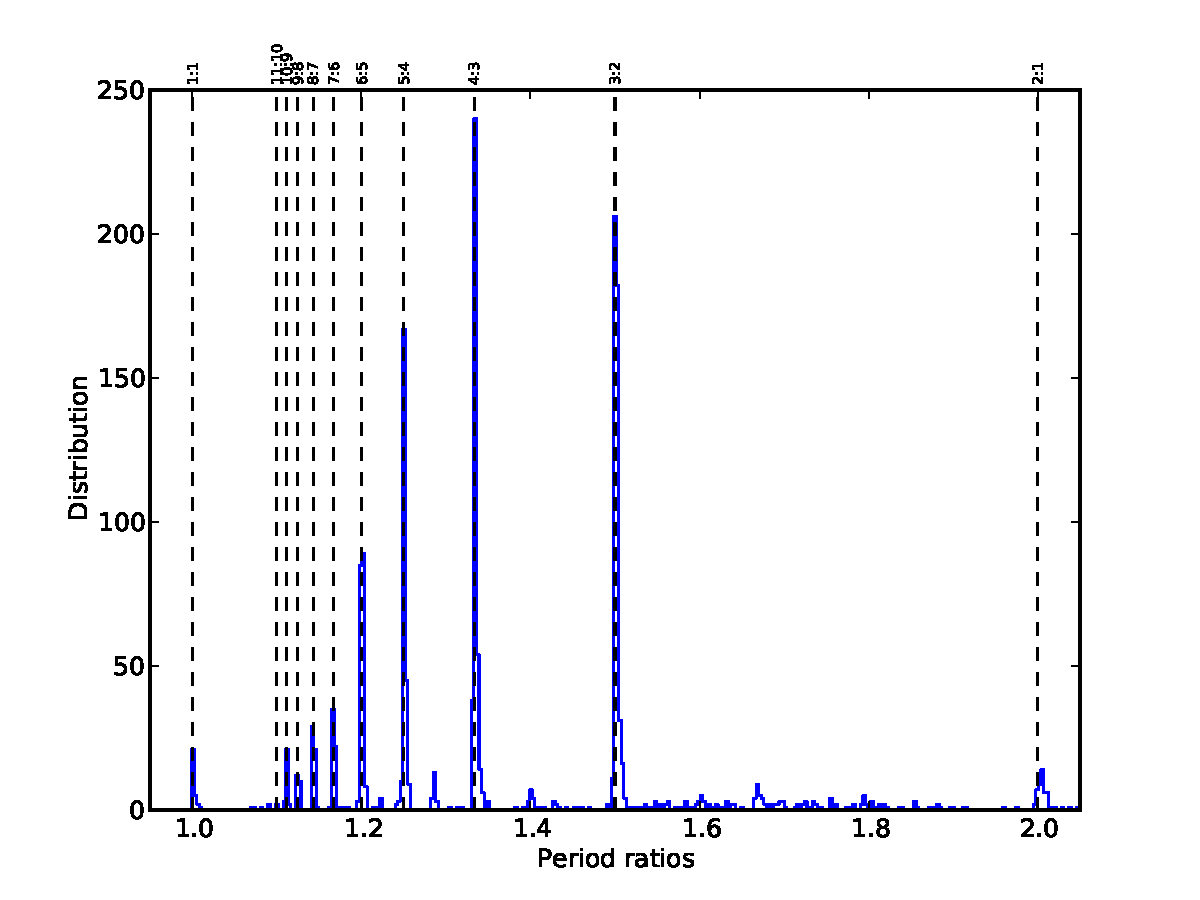
\includegraphics[width=0.49\textwidth]{figure/HSE/stat_pr_all.pdf}}\hfill
\subfloat[Masses finales]{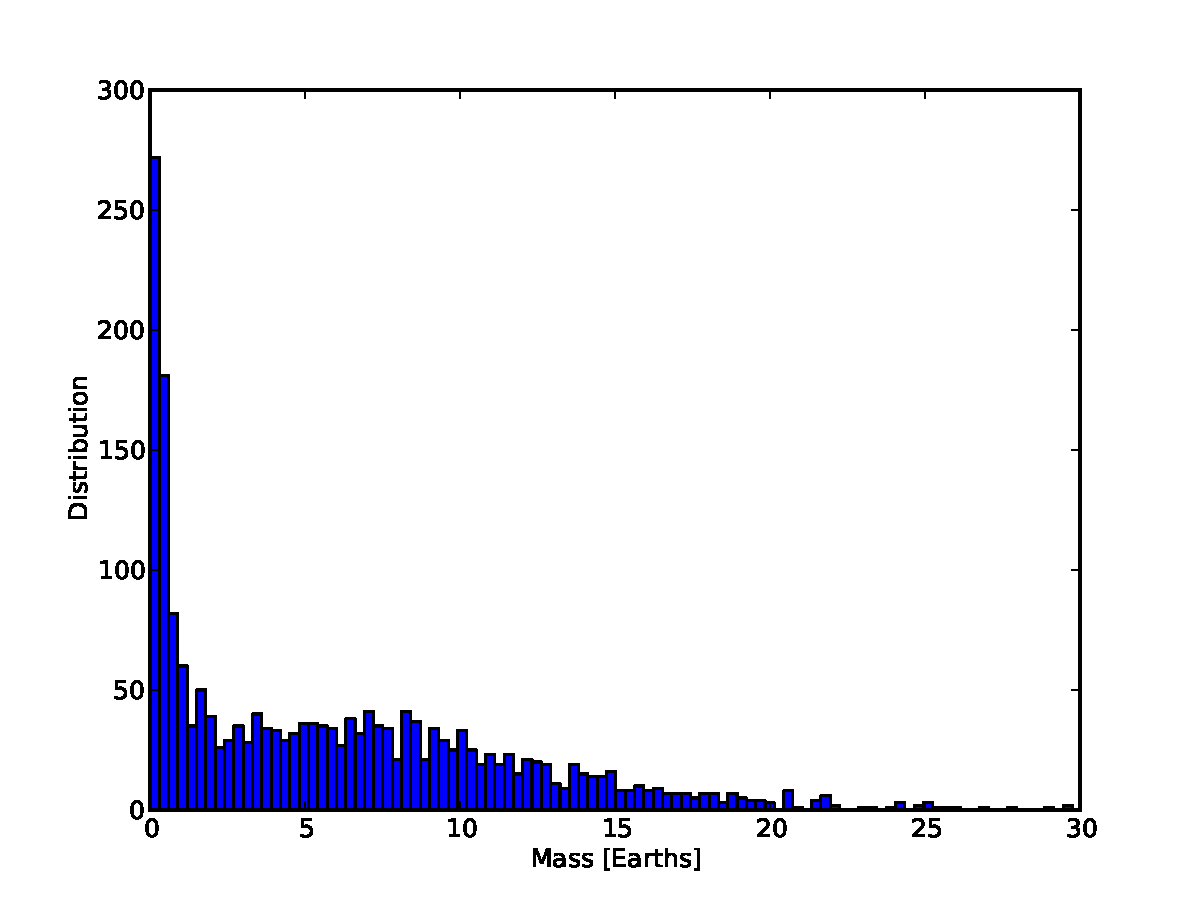
\includegraphics[width=0.49\textwidth]{figure/HSE/hist_m.pdf}}

\caption{Histogramme des rapports de période et masse des planètes pour les 200 systèmes simulés.}
\end{figure}

\begin{figure}[htbp]
\centering
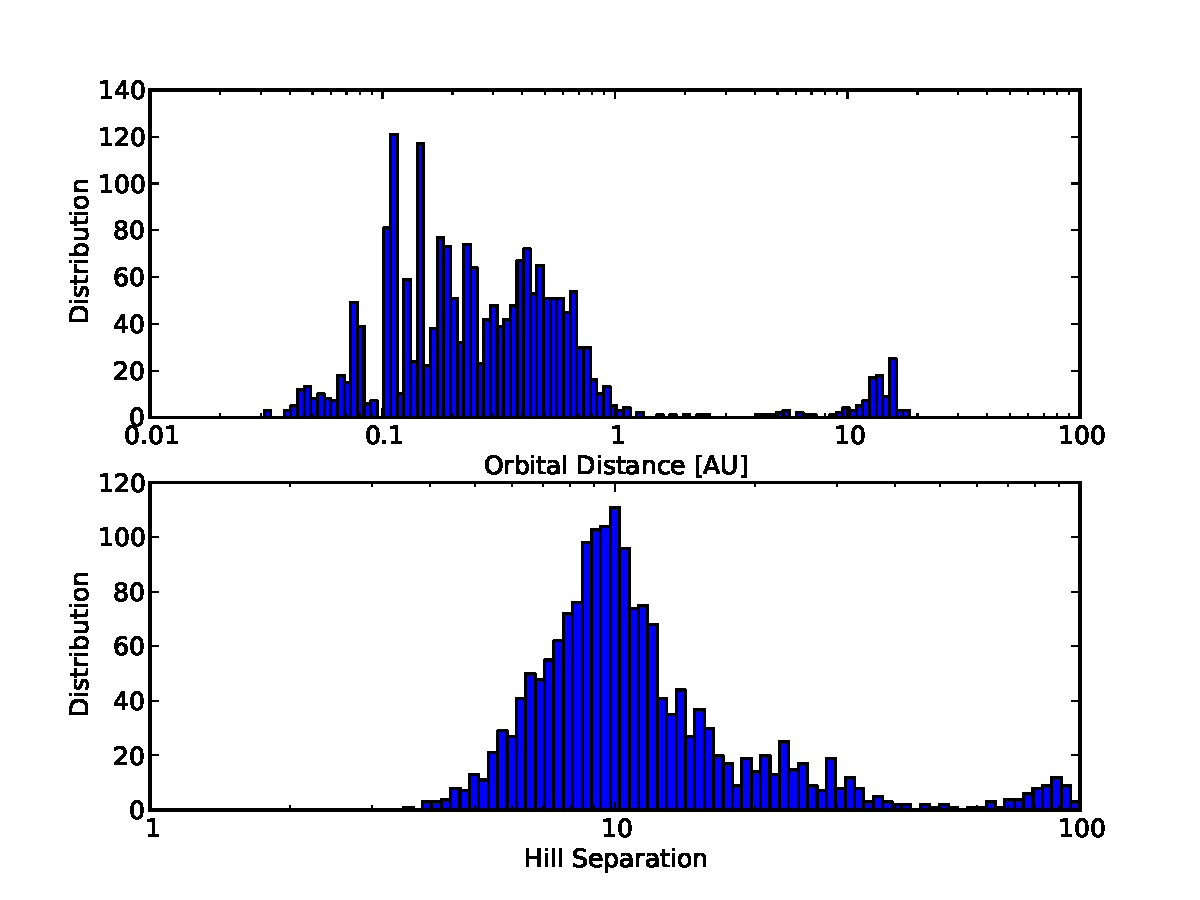
\includegraphics[width=0.7\textwidth]{figure/HSE/hist_ad.pdf}
\caption{Histogramme des positions et sép}\label{fig:HSE_stat_dist}
\end{figure}

Pour les conditions initiales décrites plus haut, nous avons simulé 200 systèmes différents. Nous cherchons maintenant à en étudier les propriétés de manière statistique. Nous observons que la plupart des planètes sont en résonance \reffig{fig:HSE_stat_pr}. La résonance la plus probable est \MMR43. Nous remarquons aussi que la grande majorité des résonances observées dans nos systèmes sont d'ordre 1. Quelques pics d'ordre $q>1$ sont visibles mais d'intensité beaucoup plus faibles que les résonances d'ordre 1 dont la visibilité a été privilégiée. 

Nous avons chercher à comparer la répartition des planètes simulées par rapport aux observations, tant au niveau de distances orbitales que des séparations en rayon de Hill mutuels \reffig{fig:HSE_stat_dist}. Ces données sont à comparer aux observations \reffig{fig:multiplanet_stats}. Les observations semblent montrer que les planètes ont plus de chance d'être séparées par $12$ rayons de Hill mutuels. Nous trouvons $10$, valeur très proche de la valeur observée dans les systèmes multiples. 

Malgré les limites du disques ($R\in[0.1;100]\unit{UA}$), nous reproduisons correctement la répartition orbitale des planètes entre $0.01$ et $1\unit{UA}$. Notons que la présence du bord interne du disque à $0.1\unit{UA}$ génère un loi bimodale autour, avec un pic avant et après le bord interne. Un fort couple de migration dans une zone du disque très restreinte pourrait expliquer la loi bimodale souvent évoquée pour représenter les observations. 

Nous avons ensuite une surdensité de planètes autour de $10\unit{UA}$ à cause de la zone de convergence qui se trouve autour de cette zone. Entre $1$ et $10\unit{UA}$ nous avons un déficit de planète dû à la migration qui entraine les faibles masses vers l'intérieur, et les masses plus importantes ($m>5\mearth$) vers l'extérieur. Les planètes ne sont donc pas stable dans cette zone. 

La migration seule, sans dissipation du disque explique relativement bien les observations au bord interne du disque, mais reproduit assez mal les planètes plus externes. Notons toutefois que nous n'avons pas modélisé l'accrétion de gaz qui doit être importante pour les embryons planétaire d'une dizaine de masses terrestres qui migrent jusqu'à $10\unit{UA}$. 

\begin{figure}[htbp]
\centering
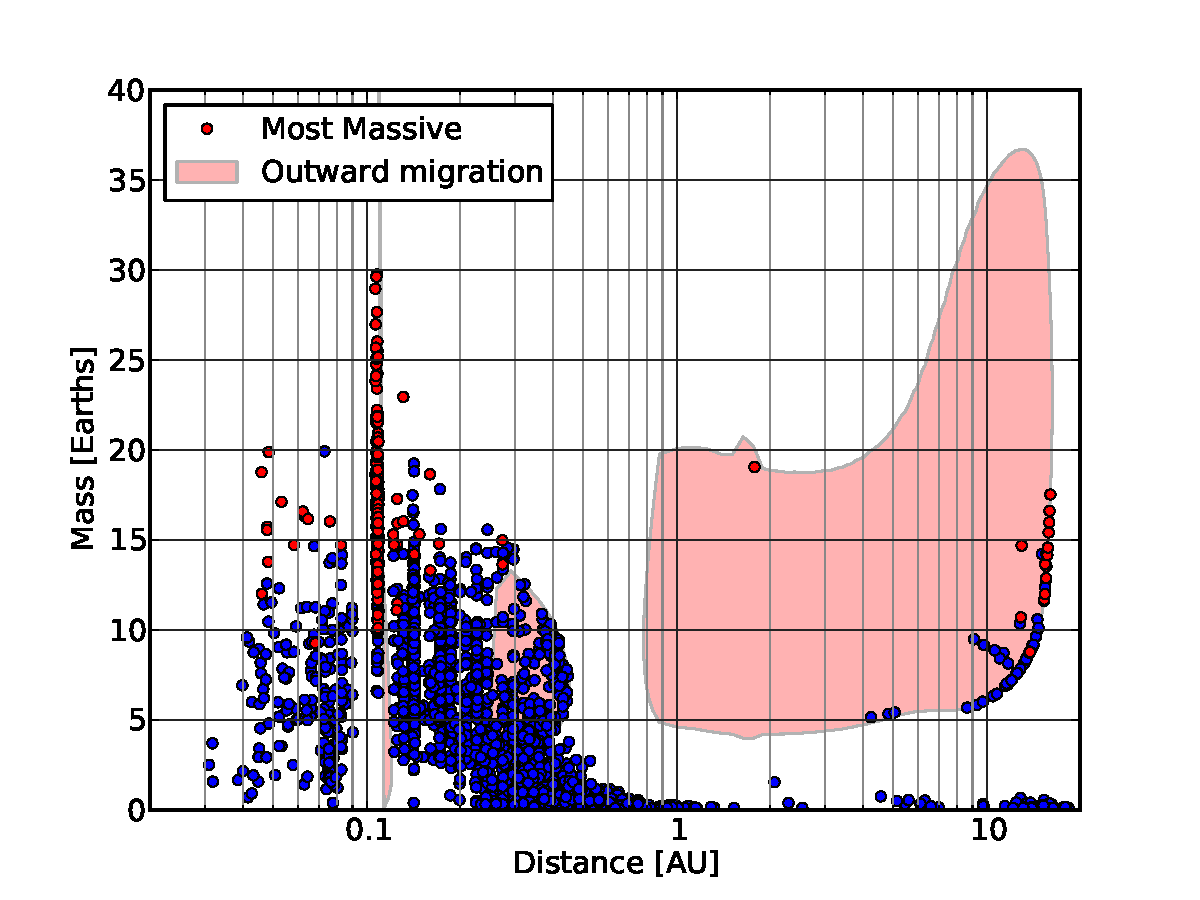
\includegraphics[width=0.8\linewidth]{figure/HSE/m_fct_a.pdf}
\caption{Position finale des planètes dans les 200 systèmes simulés dans un diagramme a-m où la carte de migration est représentée. Les planètes représentés en rouge sont chacune respectivement la plus massive d'une simulation.}\label{fig:HSE_fid_mfcta}
\end{figure}

\reffig{fig:HSE_fid_mfcta} représente sur un diagramme similaire aux cartes de migration la position finale de toutes les planètes des 200 simulations effectuées. En rouge sont représentées les planètes les plus massives de chaque simulation (200 planètes en tout) et en bleu toutes les autres planètes. Les planètes les plus massives sont essentiellement situées à des zones stables où leur couple de migration est nul. Étant les plus massives, il est difficile pour les autres planètes de les écarter de leur zone de stabilité. 

Nous avons une population de planètes au bord interne du disque ou en résonance avec une planète au bord interne. Toutes les planètes en dessous de $0.25\unit{UA}$ sont dans ce cas. Une population de planète est présente autour de chaque zone de convergence, à la fois à $0.4\unit{UA}$ et $10\unit{UA}$. À $10\unit{UA}$ nous remarquons une population de planète massives qui sont en dessous de leur zone de convergence. Ces dernières sont maintenues en deçà de leur position d'équilibre par des planètes externes en résonances qui via perturbation, amortissent leur couple de migration. En effet, cette carte ne représente que le couple de migration dans le cas où la planète ne possède pas d'excentricité. 

Les résonances se manifestent aussi par la présence, en dessous de chaque population de planète massive à une zone de résonance, d'une population de planètes peu massives à des positions où elles ne sont pas censés être stable. 

Enfin, nous avons une population de planètes qui ont été expulsées du disque au bord interne. Elles sont sur les orbites les plus internes. Leur excentricité et inclinaison ne sont plus amorties par le disque, et elles ne ressentent pas non plus de couple de migration de ce dernier. Une fois sorties du disques, les planètes peuvent continuer à migrer vers l'intérieur du disque via des résonances avec des planètes qui elles sont encore dans le disque. 

\subsubsection{Influence des paramètres initiaux}

\begin{figure}[htbp]
\centering
\subfloat[$0.1<m_i<2\mearth$]{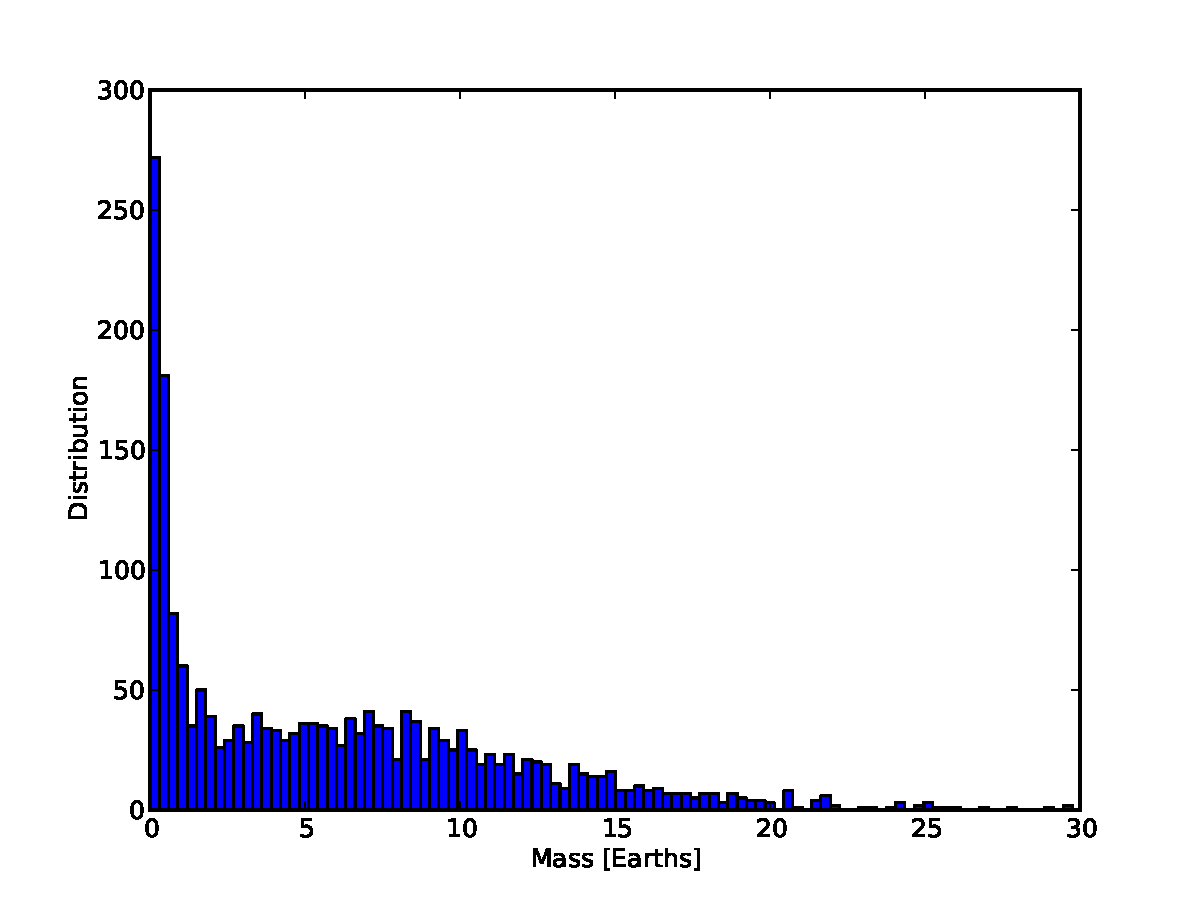
\includegraphics[width=0.49\textwidth]{figure/HSE/hist_m.pdf}}\hfill
\subfloat[$1<m_i<2\mearth$]{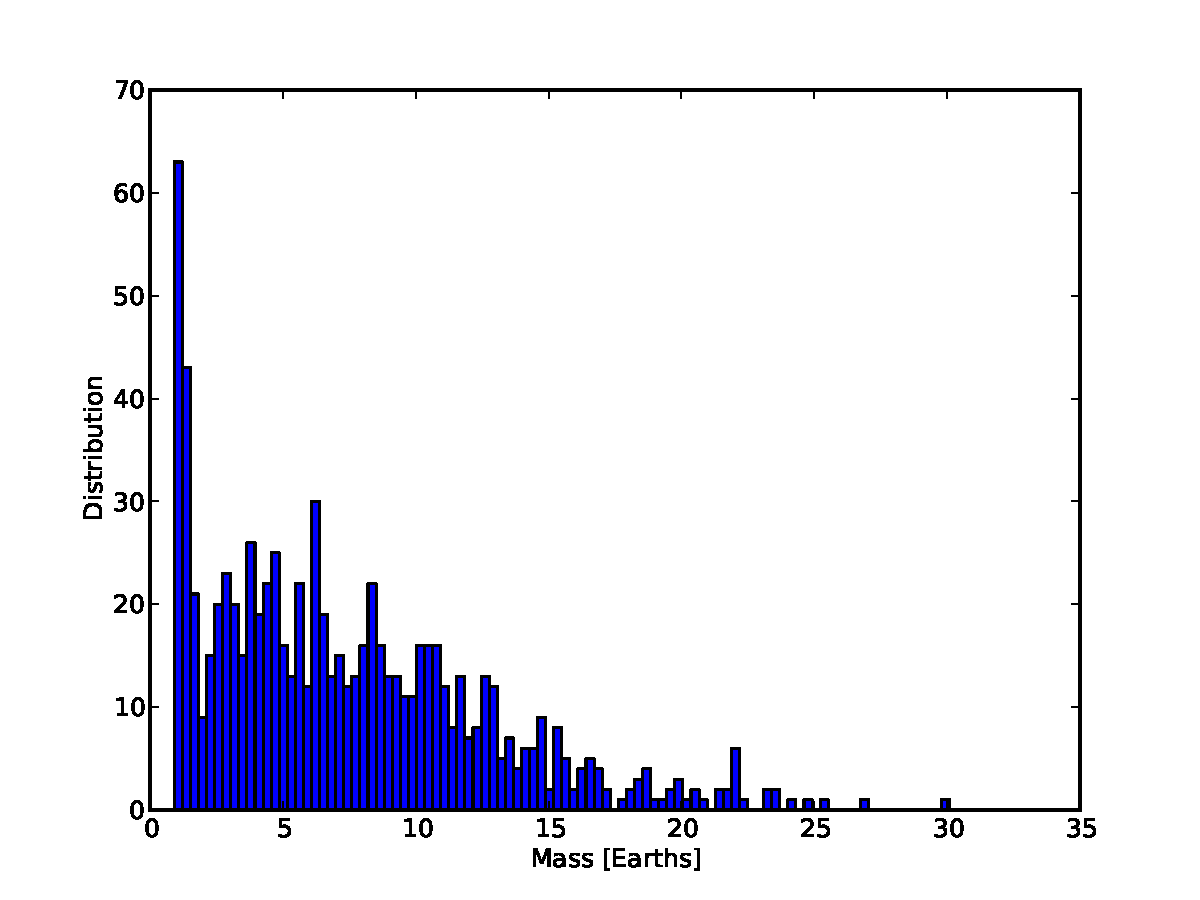
\includegraphics[width=0.49\textwidth]{figure/HSE/massive_embryos.pdf}}

\caption{Influence des masses initiales $m_i$ (la répartition est uniforme sur l'intervalle) sur la distribution des masses finales.}
\end{figure}

%TODO look at that. Must I keep this? Not very pretty to show and a bit confusing. must use normed histogram to compare things.

\subsubsection{Effet du disque}
\begin{figure}[htbp]
\centering
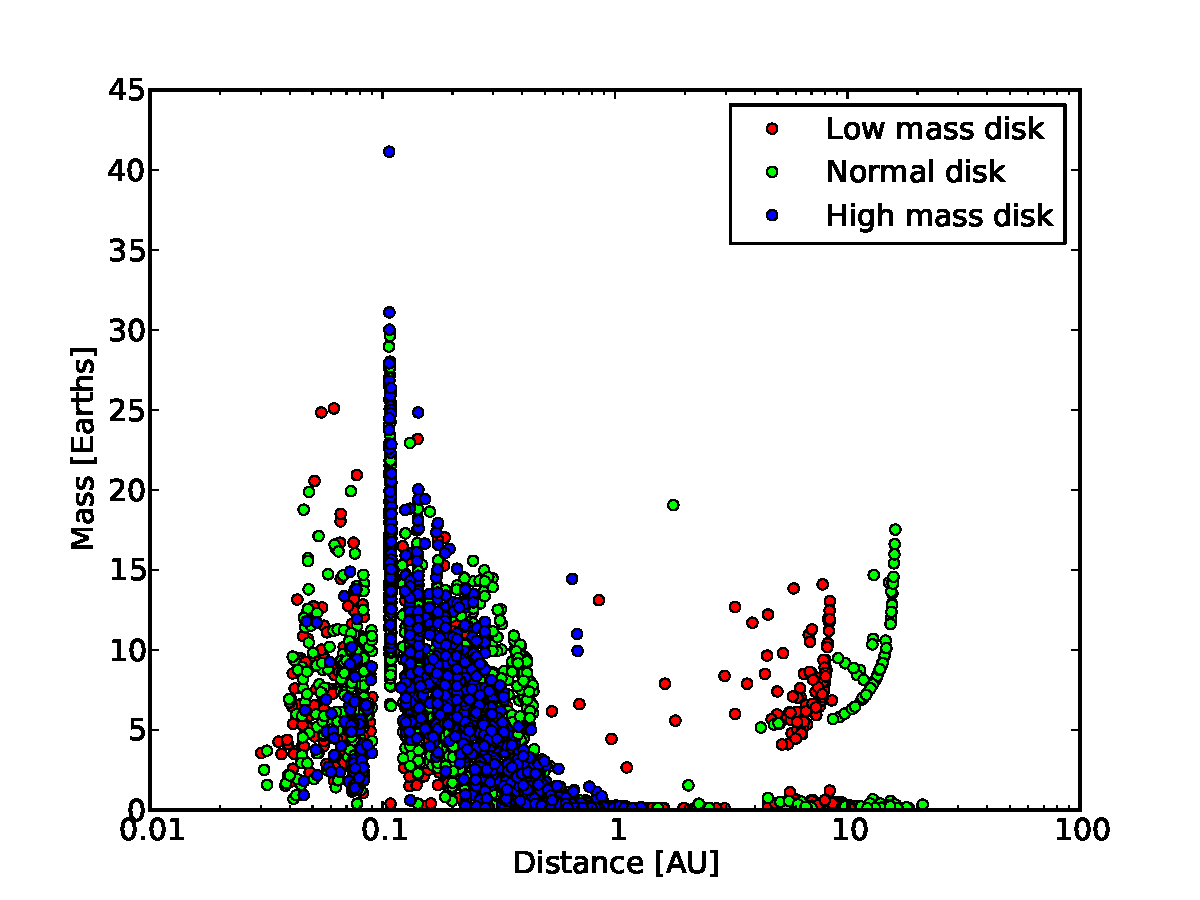
\includegraphics[width=0.8\linewidth]{figure/HSE/HSE_disk_effect.pdf}
\caption{Position finale des planètes pour différents types de disques. Le disque normal est celui présenté plus haut. Seule la masse change dans le disque de faible masse ($\Sigma_0=150\unit{g/cm^2}$) et massif ($\Sigma_0=600\unit{g/cm^2}$).}\label{fig:HSE_disk_effect}
\end{figure}

Par rapport au disque de référence où $\Sigma(R) = \Sigma_0 * R^{-\sfrac12}$, nous avons lancé 100 simulations avec un disque moitié moins massif ($\Sigma_0=150\unit{g/cm^2}$) ou moitié plus ($\Sigma_0=600\unit{g/cm^2}$) \reffig{fig:HSE_disk_effect}.

Avec le disque massif, la population de planètes au delà de $10\unit{UA}$ a disparu \reffig{fig:HSE_hist_a_disk}. Pourtant, une zone de convergence existe dans cette région, mais la masse minimale pour y accéder est de l'ordre de $10\mearth$. C'est cette augmentation de la masse critique minimale qui est la cause de l'absence de planètes au delà de $2\unit{UA}$.

Avec le disque peu massif, la population externe de planètes ($a>2\unit{UA}$) est toujours présente \reffig{fig:HSE_hist_a_disk}. La zone de convergence s'est légèrement déplacée vers l'intérieur, de l'ordre de $2\unit{UA}$ environ. Les planètes dépassent la masse critique suffisamment rapidement pour accéder à la zone de migration vers l'extérieur. De plus, la masse critique a diminué, le nombre de planètes accédant à cette zone du disque augmente donc d'autant.

\begin{figure}[htbp]
\centering
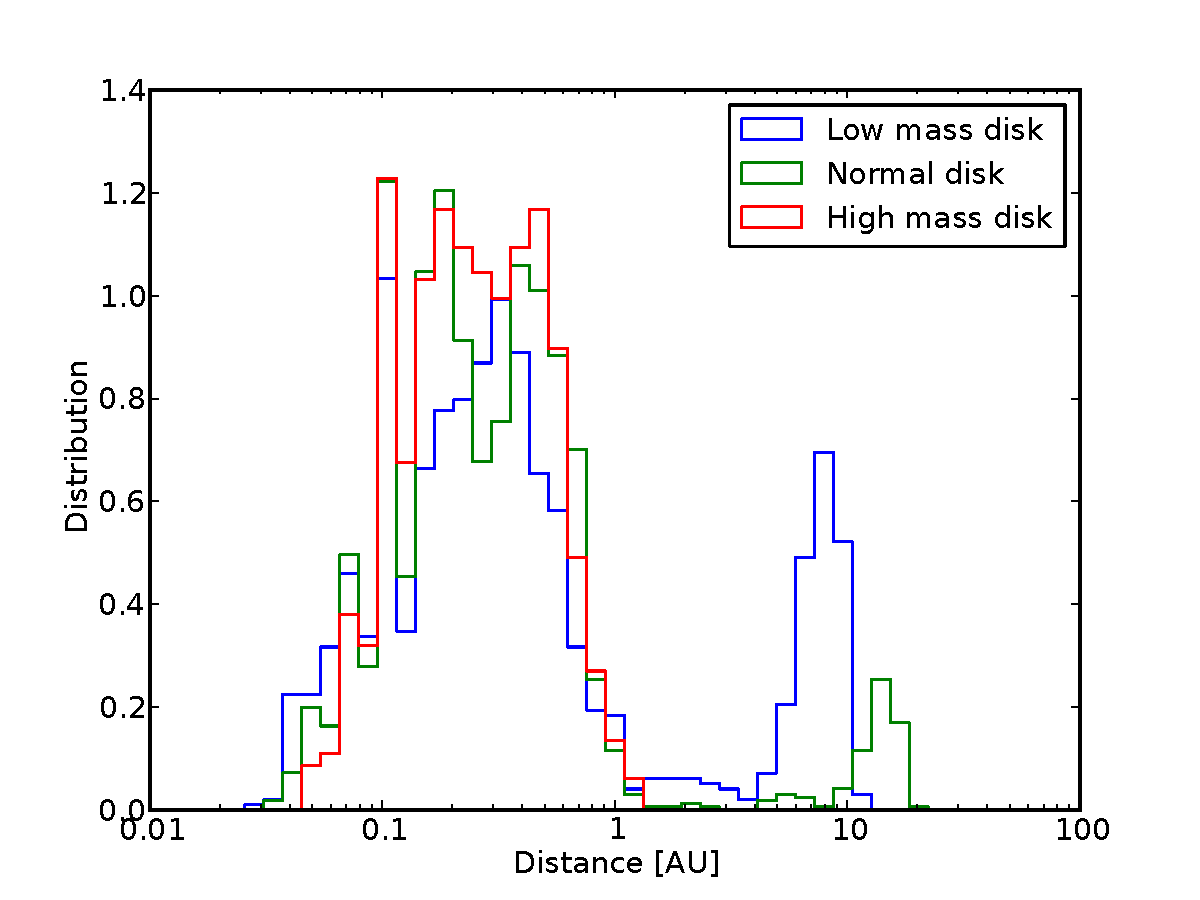
\includegraphics[width=0.8\linewidth]{figure/HSE/hist_a_disk.pdf}
\caption{Distribution des orbites finales des planètes pour trois disques différents. Seule la masse change dans le disque de faible masse ($\Sigma_0=150\unit{g/cm^2}$) et massif ($\Sigma_0=600\unit{g/cm^2}$).}\label{fig:HSE_hist_a_disk}
\end{figure}

La formation de systèmes compacts au bord interne est elle peu affectée par la variation de la masse du disque. Le fort couple positif au bord interne est stable et les planètes sont maintenues dans le disque. La distribution des positions des planètes pour la partie interne du disque $a<2\unit{UA}$ est similaire dans les trois disques. 

\subsection{Discussion}
Quand les embryons sont plus petits qu'une certaine masse critique dépendant des propriétés du disque, la migration est systématiquement vers l'intérieur. Un système compact de planètes qui grossissent par collisions se forme alors au bord interne qui retient ce système par le fort couple de corotation positif qui s'exerce juste avant le bord interne en raison de la forte décroissance de la densité de surface \citep{masset2006disk}. Au bord interne, l'onde de densité interne due au couple de Lindblad n'existe plus, étant donné qu'il n'y a plus de gaz. Le couple différentiel de Lindblad est alors simplement égal à l'onde de densité externe. La migration est malgré tout vers l'extérieur en raison du très fort couple de Corotation \citep{masset2006disk}.

Pendant la migration vers l'intérieur, si un embryon grossit suffisamment vite, il peut commencer à migrer vers l'extérieur. Durant cette migration, des résonances vont se former avec les corps qui migrent pour la plupart vers l'intérieur. Par excitation résonante, la migration vers l'extérieur peut être ralentie voire stoppée, et les planètes peuvent de nouveau migrer vers l'intérieur. 

Pourtant, dans certains cas, une planète suffisamment massive peut migrer vers l'extérieur, emprisonnant des corps plus petits dans des résonances orbitales, avant de se placer à une zone de couple nul dans les parties externes du disque (dans celui présenté ici, vers $15\unit{UA}$.

\bigskip

Ce mécanisme peut alors former conjointement des systèmes compacts de super terres, proches du bord interne, ou des cœurs de planètes géantes dans les parties externes, avec possiblement des planètes beaucoup plus petites en résonance. 

La seule différence entre le cas système compact et le cas planète géante est le timing. 

En effet, il y a deux points importants. D'une part les embryons de faibles masses migrent vers l'intérieur quelle que soit leur position initiale. De plus, les embryons en dessous d'une certaine distance migrent tous vers l'intérieur quelle que soit leur masse. Les planètes qui ne répondent pas à ces critères migreront inexorablement vers le bord interne. 

Il faut donc dans le cas présent qu'un embryon atteigne la masse critique de $5\mearth$ au delà de $1\unit{UA}$ pour pouvoir migrer vers l'extérieur et devenir un cœur de planète géante.

\bigskip

Quand nous parlons ici de système compact, il faut garder à l'esprit que le disque est toujours présent. Nous ne faisons pas évoluer le disque au cours du temps, la dissipation aura donc certainement un effet. Les résonances, présentes systématiquement au bord interne à cause de la migration, auront des chances de disparaître si des déstabilisations surviennent pendant la dissipation. En effet, le système n'est stable qu'à cause de la dissipation induite par le disque de gaz. Pourtant, il est difficile de conclure car la manière dont le disque est dissipé aura une incidence sur la configuration finale du système. 

Ensuite, nous n'avons pas tenu compte de l'accrétion de gaz sur les super terres. D'un coté des planètes de plusieurs masses terrestres vont pouvoir accréter du gaz, mais la proximité de ces planètes à leur étoile centrale pourra avoir une effet dissipatif sur leur atmosphère. 

Ensuite, \cite{terquem2007migration} ont montré que la formation de systèmes compacts est possible. Ici, le modèle que nous avons repris est très similaire à leur modèle, à ceci près que nous avons modélisé la migration de manière consistante avec le disque (avec possibilité de couple positif et négatif en fonction de la masse et de la position de la planète). 

Ce que notre modèle montre en plus du modèle de \cite{terquem2007migration} (voir aussi \cite{ogihara2007accretion,
cresswell2008three}), c'est que même avec migration vers l'extérieur, des systèmes compacts peuvent se former au bord interne,
avec des propriétés très similaires aux propriétés des systèmes observés. Mais de plus, dans le même modèle, la formation de
cœurs de planètes géantes dans les parties externes est possible. 

